\documentclass[12pt]{article}

\usepackage{hyperlatex}
\usepackage[pdftex]{graphicx}

\T \topmargin      0.0in
\T \headheight     0.0in
\T \headsep        0.0in
\T \oddsidemargin  0.0in
\T \evensidemargin 0.0in
\T \textheight     9.0in
\T \textwidth      6.5in

\newcommand{\HlxIcons}{../images/}

\htmltitle{GraspIt! User Manual}
\htmladdress{Copyright (C) 2002-2009 Columbia University}

\htmldirectory{../html-manual}
\htmlname{graspit-manual}
\htmlpanelfield{Contents}{hlxcontents}

\setcounter{htmldepth}{2}
\setcounter{htmlautomenu}{2}
\setcounter{secnumdepth}{2}
\setcounter{tocdepth}{2}

\title{
%GraspIt!
\texorhtml{
\centerline{

\includegraphics[width=50mm]{../images/logo.jpg}}
}
{\htmlimg{../images/logo.jpg}\\
}
User Manual}
\date{Version 2.2}

\begin{document}
\label{hlxcontents}

\maketitle

\T \tableofcontents

\texonly{\newpage}

\section{Introduction}

\htmlmenu{2}

\subsection{What GraspIt! is}

GraspIt! was created to serve as a tool for grasping research. It is a
simulator that can accommodate arbitrary hand and robot designs. It
can also load objects and obstacles of arbitrary geometry to populate
a complete simulation world. The GraspIt! engine includes a rapid
collision detection and contact determination system that allows a
user to interactively manipulate a robot or an object and create
contacts between them. Once a grasp is created, one of the key
features of the simulator is the set of grasp quality metrics. Each
grasp is evaluated with numeric quality measures, and visualization
methods allow the user to see the weak point of the grasp and create
arbitrary 3D projections of the 6D grasp wrench space.

In our experience, we have found that GraspIt! usually serves one of
two purposes. First, it can be used as a development tool, to execute
and test various robot control algorithms. In this sense, it serves as
a replacement for the real world: in simulation, an algorithm can be
tested on many hand designs, many objects and obstacle configurations,
at no cost and much faster than in the real world. Second, GraspIt!
can be used as a computational platform that backs up a robot that
does operate in the real world. For example, a real robot can acquire a
model of a target object, then use GraspIt! to quickly evaluate
multiple grasping or manipulation scenarios. Often, these scenarios
are also combined and the same GraspIt! setup used for development of
an algorithm can also be used for computations during real life
execution.

GraspIt! has many features that help accomplish these roles; all of
these features are documented in the second part of this manual. The
most commonly used include the contact detection and grasp quality
metrics mentioned above, the dynamics engine and the grasp planning
capabilities. The dynamics engine within GraspIt! computes the motions
of a group of connected robot elements, such as an arm and a hand,
under the influence of controlled motor forces, joint constraint
forces, contact forces and external forces. This allows a user to
dynamically simulate an entire grasping task, as well as test custom
robot control algorithms. The grasp planning algorithms rely on the
simulated environment to quickly evaluate many hand postures, and
find those that lead to stable grasps. There are many possible
implementations of this concept; the planners that are included with
GraspIt! can usually find multiple stable grasps of an object in less
than 1 minute, taking into account obstacles and other constraints.

Overall, GraspIt! is an open-source virtual environment for simulating
robotic grasping tasks accompanied by a number of analysis and
development tools. It has been developed in C++ using many other
open-source libraries, and is cross-platform, tested on both Windows
and Ubuntu Linux.

\subsection{What GraspIt! is NOT}

GraspIt! is not an off-the-shelf product. It is rather a large
codebase that is the result of many years of research and development
in the Robotics Lab at Columbia University. The tools included can
greatly help in the development and testing of new algorithms and
approaches. However, we have often found that most new interesting
problems can not be completely addressed by applying these tools
exactly as they are. It is very possible that, in the process, you
will find yourself needing various changes or additions to the
simulator; these might be bigger or smaller depending on your
problem. This means that you might have to get your hands dirty and
tinker with the code itself, which we encourage you to do. We have
done our best to create clean, robust and well-documented
code. However, we are not a large team of product development software
engineers; rather, we are a small group of robotics researchers. As a
result, do not be surprised if you find parts of the code that can be
improved.

\subsection{About this manual}

This manual is divided into two parts. The first one, containing
\textbf{Chapters 1 through 4}, is an introduction to the GraspIt!
environment, covering the essential aspects for loading and populating
a GraspIt!  world and interacting with it. The references to the
source code are kept at a minimum. In the second part, containing
\textbf{Chapters 5 through 17}, we discuss the GraspIt! advanced
features, or the tools that it offers for solving various
problems. Here we overlap discussions of the simulator as a final
product with discussion of the source code itself. We also introduce a
number of features of GraspIt!  that are not completely finished yet,
and might not be very robust, but have been included in the
distribution in the hope you might find them useful. Such features
will be marked by the qualifier "Under Development" - only use them if
you're not afraid of delving inside the code to get the most out of
them and fix an occasional bug.

Please note that, much like the code itself, this manual is under
continuous development. There are many aspects that it does not touch
at all, or explains too briefly. If there is a topic that you found
particularly confusing, or you would like to see expanded, we would
appreciate your feedback.

\subsection{Troubleshooting and contact}

GraspIt! includes two main resources: this manual, and a complete code
reference. We have put a lot of work into both of them, and we
strongly encourage you to try using them to solve your problem before
contacting us. If that fails, we will try to provide support via
email; write us at \texttt{graspit@lists.cs.columbia.edu}. General comments
on the simulator, and any patches or improvements to the code are
always appreciated.

\subsection{Authors and acknowledgements}

\textbf{Andrew Miller} and \textbf{Matei Ciocarlie} are the main
authors of GraspIt!, having designed most of its features and
implemented most of the code. GraspIt!'s current main developers and
maintainers are Matei Ciocarlie and \textbf{Jon Weisz}. The GraspIt!
simulator was developed in the Robotics Lab, Department of Computer
Science, Columbia University, under the guidance of
\textbf{Prof. Peter Allen}.

Many people contributed to GraspIt!, either in the form of new ideas,
suggestions or guidance, or by implementing new features in
code. These include: \textbf{Prof. Jeff Trinkle}, who provided
valuable advice on the dynamics system; \textbf{Danica Kragic} who
developed the real time vision system allowing GraspIt! to work with
real robots; \textbf{Prof. Henrik Christensen} and \textbf{Steffen
  Knoop} who helped build the automatic grasp planner; \textbf{Raphael
  Pelossof}, who implemented the first GraspIt! based machine learning
approach; \textbf{Claire Lackner}, who helped design and implement the
soft finger contact algorithms; \textbf{Corey Goldfeder}, who was the
driving force behind the Columbia Grasp Database (CGDB) which is now
integrated with GraspIt!; \textbf{Hao Dang} who wrote the GraspIt! -
CGDB interface, and made many other valuable contributions to the
codebase; \textbf{Norases Vesdapunt}, who wrote the XML interface for
data files. We would like to thank all of them for their valuable
contributions.

Thanks to Prof. Gerd Hirzinger and Dr. Max Fischer, Prof. Contantinos
Mavroidis and Katheryn DeLaurentis, Dr. Myron Diftler, Marco Reichel,
the Shadow Robot Company, Marius Stuecheli and Dr. Tamim Asfour for
providing us with models of their robotic hands. The M7 Robot geometry
was provided courtesy of SRI International. The Schunk Dexterous Hand
model was provided courtesy of SCHUNK GmbH Co. The RobotIQ hand
model was provided courtesy of the RobotIQ Company.

We would also like to thank \textbf{Willow Garage} for their support
towards this new, GPL-licensed release, and for their commitment
towards open-source and freely available code.

\section{Installation}

\htmlmenu{2}

The GraspIt! installation process consists of two steps. First, you
must install a set of external libraries, listed below. The
installation for each library is further detailed in the system
specific sections of this installation guide. Then, you must compile
the GraspIt! code itself and set up the environment variables.

GraspIt! needs the following external libraries:

\begin{description}
\item[Qt] Qt is a cross-platform application and UI framework. It
  allows GraspIt! to have a platform-independent windowing system,
  dialogs etc. GraspIt! currently uses Qt version 4, which is
  available under two different licenses. This installer assumes you
  will be using the open source version, see the \xlink{Qt
    website}{http://www.qtsoftware.com} for more details on licensing
  options.

\item[Coin] Coin is a Scene Graph API that GraspIt! uses for all of
  its 3D rendering needs. It is an Open Inventor clone. At this time,
  the latest version of Coin is Coin 3, but due to some compatibility
  problems we advise using Coin 2 with GraspIt!. Like Qt, Coin is
  available under a dual licensing model; here we assume you will be
  using the open source license. See the
  \xlink{Coin3D}{http://www.coin3d.org} website for more licensing
  details.

\item[SoQt] SoQt is a GUI binding, essentially the "glue" between Qt
  and Coin. It is available, under the same conditions as Coin, from
  the Coin website. The latest version of SoQt that we have tested
  GraspIt! with is SoQt 1.4.1, which provides seamless integration
  with Qt4.

\item[Lapack] Lapack is a library for scientific computing that
  GraspIt! uses for various matrix related tasks, such as matrix
  multiplication, linear system solving, singular value decomposition,
  etc.
\end{description}

The GraspIt! project information comes in the form of a cross-platform
Qt project file, which is processed by QMake. Depending on your
system, you will convert this into either a Makefile or a Microsoft
Visual Studio project file.

\subsection{GraspIt! Installation - Ubuntu Linux}

\subsubsection{Qt}

You will need the following libraries in order to compile GraspIt!:
\begin{itemize}
\item Qt 4
\item Coin 3
\item SoQt
\item Blas and Lapack
\end{itemize}

On Ubuntu, you should be able to get all these from the package
manager. It should also possible to compile them all from code, but
since that tends to be system-specific we no longer provide
instructions or guidelines for that.

Use \texttt{sudo apt-get install} to install the following packages:
\begin{itemize}
\item \texttt{libqt4-dev}
\item \texttt{libqt4-opengl-dev}
\item \texttt{libqt4-sql-psql}
\item \texttt{libcoin60-dev}
\item \texttt{libsoqt4-dev}
\item \texttt{libblas-dev}
\item \texttt{liblapack-dev}
\end{itemize}

\subsubsection{GraspIt!}

Download and unzip the GraspIt! code itself. Set the following
environment variable:

\begin{itemize}
\item \texttt{GRASPIT} - the directory where you unzipped GraspIt!
\end{itemize}

Build QHull. Go to the \texttt{\$GRASPIT/qhull} directory and type
\texttt{make}.

Create the GraspIt! Makefile from the Qt project file. Edit
\texttt{\$GRASPIT/graspit.pro} to suit your system and
installation needs. Then type \texttt{qmake graspit.pro}.

Build and go. From \texttt{\$GRASPIT/} type \texttt{make}.

\subsection{GraspIt! Installation - Windows}

We assume you are using the Microsoft Visual Studio compiler. Some of
the paths provided as examples in this installer are taken from MS
Visual Studio 2003; the change to your particular version of the
compiler should be straightforward.

\subsubsection{Qt}

Download Qt for C++ from the the \xlink{Qt
  website}{http://www.qtsoftware.com/downloads}.

GraspIt! is currently tested using Qt 4.5.2. So far, we have had the
best experience with \textbf{the source code version of Qt}, NOT any
of the installers that come with pre-built binaries. On the Qt
website, choose "Qt: Framework Only", then "Download Qt libraries 4.5
for Windows (166 Mb)" and finally click the link under "Source code
available on this link:". Currently, the recommended download link
that you will arrive at is
\xlink{http://get.qtsoftware.com/qt/source/qt-win-opensource-src-4.5.2.zip}{http://get.qtsoftware.com/qt/source/qt-win-opensource-src-4.5.2.zip}. However,
this will change as new versions are added to the website. Unzip the
archive to a directory of your choice.

Set the following environment variables:

\begin{itemize}
\item \texttt{QTDIR} - the directory where you unzipped Qt (e.g. \texttt{C:/Qt/4.4.3})
\item \texttt{QMAKESPEC} - this has to be set depending on your c++
  compiler and platform. See \texttt{\$QTDIR/mkspecs} for a list of
  options. If using Microsoft Visual Studio 2003, set this variable to
  \texttt{win32-msvc2003}.
\item \texttt{PATH} - add \texttt{\$QTDIR/bin} to your \texttt{PATH}
\end{itemize}

You might also need to add to some compiler-specific paths to your
environment variables. If Qt's configure script fails, try to look
what file it failed to find, then add the respective path to either
\texttt{PATH}, \texttt{INCLUDE} or \texttt{LIB}. Also be aware of where in the particular environment variable you add a certain path - when searching for a
file, the system will use the first one that it finds, which might not
be the one that you intended. Here are, as examples, the paths that
need to be added when using MS Visual Studio 2003:

\begin{itemize}

\item \texttt{PATH}:
\begin{itemize}
\item the path to \texttt{nmake.exe} (e.g. \texttt{C:/Program Files/Microsoft Visual Studio .NET 2003/Vc7/bin} )
\item the path to the common dlls (e.g. \texttt{C:/Program Files/Microsoft Visual Studio .NET 2003/Common7/IDE} )
\end{itemize}

\item \texttt{INCLUDE}:
\begin{itemize}
\item \texttt{C:/Program Files/Microsoft Visual Studio .NET 2003/Vc7/include}
\item \texttt{C:/Program Files/Microsoft Visual Studio .NET 2003/Vc7/PlatformSDK/Include}
\end{itemize}

\item \texttt{LIB}:
\begin{itemize}
\item \texttt{C:/Program Files/Microsoft Visual Studio .NET 2003/Vc7/PlatformSDK/Lib}
\item \texttt{C:/Program Files/Microsoft Visual Studio .NET 2003/Vc7/lib}
\end{itemize}

\end{itemize}

Follow the instructions provided with the Qt distribution for
installing (note: installation might take a couple of hours). We
recommend building both release and debug versions of Qt, so you have
all your options for linking later
on. Use \texttt{configure~-debug-and-release} for that.

WARNING: Other programs use Qt binaries, and often include the Qt
dll's (such as \texttt{QtGui4.dll}) in their distribution. If a path
to some other version of a Qt dll exists in you \texttt{PATH}
environment variable \textbf{before} \texttt{\$QTDIR/bin}, the system
will link GraspIt against the wrong version, often causing failure to
run. To be sure that you are linking against the right dll's, put
\texttt{\$QTDIR/bin} at the beginning of your \texttt{PATH}.

\subsubsection{Coin}

Download Coin3d for your C++ compiler from the \xlink{Coin3D
website}{http://www.coin3d.org}.

We have tested the installation of GraspIt! using Coin 2.4.6. If using
MS Visual Studio 2003, we recommend downloading Coin 2.4.6 VC7
binaries, no installer.

Set the following environment variables:

\begin{itemize}
\item \texttt{COINDIR} - the directory where you unzipped Coin (e.g. \texttt{C:/Coin3D/2.4.6}).
\item \texttt{PATH} - add the path to \texttt{coin2.dll} (e.g. \texttt{C:/Coin3D/2.4.6/bin}).
\end{itemize}

\subsubsection{SoQt}

Download SoQt from the \xlink{Coin3D website}{http://www.coin3d.org}.

You will need to build SoQt yourself from source code. The source code
comes with MS Visual Studio solution files, choose the appropriate one
depending on your compiler. Again, we recommend building both debug
and release versions. After the build completes, take a look in
\texttt{\$COINDIR/bin} to make sure that the appropriate SoQt dlls (\texttt{soqt1.dll} and/or \texttt{soqt1d.dll}) have been built.

\subsubsection{Lapack}

You will need to link GraspIt! against your favorite implementation of
Lapack. This usually involves two steps: using a ``wrapper'' file so
you can call Fortran functions from C code and linking against the
correct library.

We have tested GraspIt! with two Lapack implementations:
\begin{itemize}
\item Intel Math Kernel Library (MKL), available from
  \xlink{http://software.intel.com/en-us/intel-mkl/}{http://software.intel.com/en-us/intel-mkl/}
  (free trial available);
\item CLapack, available from
  \xlink{http://www.netlib.org/clapack/}{http://www.netlib.org/clapack/}.
\end{itemize}

If you install one of these two, you can use them as follows:
\begin{itemize}
\item set the environment variable \texttt{MKLDIR} or
  \texttt{CLAPACKDIR} to the root of the respective Lapack library
  installation;
\item set the appropriate flag in the main GraspIt! project file (see below).
\end{itemize}

Unfortunately, it is possible that you might have to change these
settings to get the installation to work on your system, or you might
be using a different version of Lapack altogether. Due to the large
number of possible configurations, we can not provide more in-depth
guidelines. If linking against Lapack fails, please see the
Windows-specific GraspIt! project file
(\texttt{graspit-lib-WINDOWS.pro}), find the blas/lapack block, and
try to adapt it to your settings.

\subsubsection{GraspIt!}

Download and unzip the GraspIt! code itself. Set the following
environment variable:

\begin{itemize}
\item \texttt{GRASPIT} - the directory where you unzipped GraspIt! (e.g. \texttt{C:/Documents and Settings/your\_username/My Documents/Graspit}).
\end{itemize}

Build QHull. Open and build the MS Visual Studio solution
\texttt{\$GRASPIT/qhull/windows/qhull.sln}. Once again, we recommend building
both debug and release versions. Make sure \texttt{qhull.lib} has been
installed in the appropriate directory
(\texttt{\$GRASPIT/qhull/windows/Debug}
and/or \texttt{\$GRASPIT/qhull/windows/Release}).

Edit \texttt{\$GRASPIT/graspit.pro} to suit your particular
installation. Among other options, you can choose which version of
Lapack to use. Then, create the GraspIt! MS Visual Studio project file
from the Qt project file. Execute the following command from inside
\texttt{\$GRASPIT} in a command prompt:

\texttt{qmake -t vcapp -o graspit.vcproj graspit.pro}

This will create your GraspIt! MS Visual Studio project file. Open
\texttt{graspit.vcproj} in MS Visual Studio. Build GraspIt! and run.

\textbf{IMPORTANT}: 
based on the choice of Debug vs. Release made in
the \texttt{graspit.pro} file, make sure the appropriate configuration
(Debug or Release) is \textbf{also} selected in MS Visual Studio. This
ensures linking against the correct Qt libraries.

\textbf{WARNING}: it is not enough to switch between Debug and Release builds
using only the option in in MS Visual Studio. This will link against
the appropriate Qt libraries but NOT against the appropriate Coin,
SoQt and QHull libraries! The correct way of choosing a Debug or
Release build is to also edit the \texttt{graspit.pro} file.

\section{Getting Started}

\htmlmenu{2}

\newcommand{\myimg}[1]{\texorhtml{\includegraphics[width=5mm]{../images/#1}}{\htmlimg{../images/#1}}\ }

To get started, use the File $\rightarrow$ Open menu, and load the
simulation world file \texttt{dlr\_flask.wld}. Note that by default
GraspIt!  will look for world files in \texttt{\$GRASPIT/worlds}. This
is a very simple simulation world containing nothing except a hand
(the DLR model) and an object (a flask).

\begin{figure}[h]
\texorhtml{
\centerline{
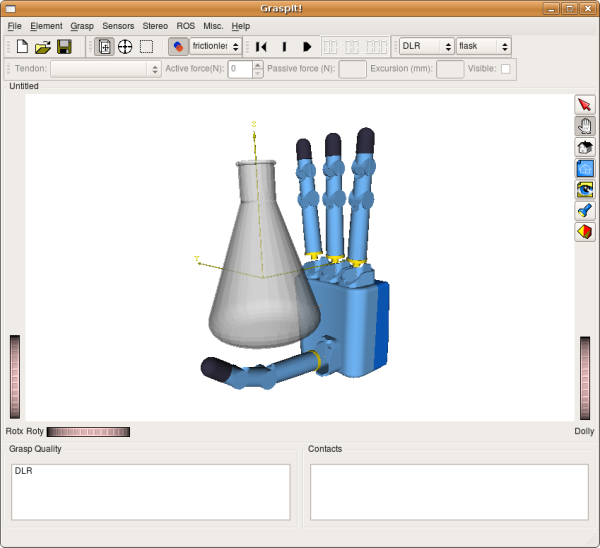
\includegraphics[width=5.0in]{../images/dlr_flask.png}}
}
{\htmlimg{../images/dlr_flask.png}
}
\end{figure}

In general, you can also start with an empty simulation world and
populate it by importing robots and objects, one at a time, using the
Import options in the File menu. You can then save a simulation world
into a world file, like the one that we just opened. In this quick
tutorial, we will be using a couple of simulation worlds supplied with
the distribution.

\subsection{The main window and controls}

The most part of the GraspIt! main window is occupied by the Inventor
viewer, which renders the virtual world. On the right side there is a
vertical toolbar: this is the Inventor toolbar which is responsible
for camera interaction.

The first two buttons on the Inventor toolbar determine which state
the viewer is in. When \myimg{arrowTool.jpg} is selected, the viewer
is in \textbf{Interaction mode}. This is the only mode in which you
can interact with the objects in the simulation world. When
\myimg{handTool.jpg} is selected, the viewer is in \textbf{Camera
  mode}. This is the only mode in which you can move the camera.

You can also toggle between \textbf{Interaction mode} and
\textbf{Camera mode} by pressing the \texttt{<ESC>} or \texttt{<ALT>}
keys, although this seems not to work on all systems.

\subsubsection{The Camera mode}

When the viewer is in \textbf{Camera mode}, you can move the virtual
camera in the following ways:
\begin{itemize}
\item \textbf{Rotate} - Hold down the left mouse button and drag;
\item \textbf{Translate} - Hold down \texttt{<CTRL>} and the left
  mouse button and drag; alternatively, hold down the middle mouse
  button and drag;
  \item \textbf{Zoom} - Hold both the left and middle mouse buttons
    and drag, or rotate the wheel on a wheel mouse.
\end{itemize}

In addition, the following buttons on the Inventor toolbar are useful:
\begin{itemize}
\item \myimg{viewAllTool.jpg} - This automatically moves the camera so
  that the entire scene fits in the viewer window;
\item \myimg{seekTool.jpg} - The seek tool allows you to click on an
  object in the scene. After you click, the camera zooms in on the
  object, which also becomes the center of rotation.
\end{itemize}

Take a moment to move the camera around and familiarize yourself with
its controls.

\subsubsection{The Interaction mode}

When the viewer is in \textbf{Interaction mode}, you can interact with
the objects in the scene. The type of interaction is determined by the
following button in the GraspIt! toolbar: \myimg{translateTool.jpg}
\myimg{rotateTool.jpg} \myimg{selectTool.jpg}:

\begin{itemize}
\item \myimg{translateTool.jpg} - \textbf{Translate or set
  joints}. Clicking on a body or the base (palm) of a robot causes a
  box to be drawn around it. This box acts as a translation
  manipulator. By clicking on the sides of the box and dragging the
  mouse, the body or robot can be translated in 2 dimensions that are
  aligned with the face of the box that was clicked. Holding down
  \texttt{<SHIFT>} constrains this motion to one axis. If a robot is
  selected and moved.

  Clicking on a kinematic chain causes joint draggers to be drawn for
  each DOF on that chain. You can then use these draggers to move the
  joints of the robot.
\item \myimg{rotateTool.jpg} - \textbf{Rotate}. Clicking a body or
  robot base link brings up a spherical rotation manipulator. Dragging
  the ball allows rotation of the selected item in three
  dimensions. By clicking one of the stripes, the body can be rotated
  about one axis at a time. By dragging the cross hairs, the ball can
  be re-centered to rotate about a different point. The limitations
  concerning connected robots applies to rotation as well.
\item \myimg{selectTool.jpg} - \textbf{Select}. Clicking a body will
  select it, and this is indicated with a wireframe overlay. Holding
  down \texttt{<SHIFT>} allows multiple bodies to be selected, or
  clicking on an already selected link of a robot will select the
  whole robot. Once a body (or bodies) has been selected, its
  collision and material properties are shown in the next part of the
  toolbar. They can then be changed or additional properties can be
  changed using the menu item described below. After a body is
  selected, the user may remove the body from the world by pressing
  \texttt{<DEL>}.
\end{itemize}

Try to use the \myimg{translateTool.jpg} tool to flex the fingers of
the robot. Note that once a finger touches the object, a contact is
marked and no more flexion is allowed. The same behavior applies for
moving objects or robots around.

The following buttons in the GraspIt! toolbar apply to the currently
selected body (if any):
\begin{itemize}
\item \myimg{collide.jpg} - \textbf{Toggle Collisions}. There are 3
  different ways to use this property:
\begin{itemize}
\item if no body is selected, this button allows collision checking
  for the entire world to be switched on or off.
\item if one or more than two bodies are selected, this button sets
  the collision checking for those bodies. A body that has collision
  checking turned off can pass through ANY other body.
\item if two bodies are selected, this button allows collision
  checking between ONLY that pair of bodies to be disabled.
\end{itemize}
\item \myimg{materialSelect.jpg} - \textbf{Material}. This sets the
  material for the selected bodies, which affects the coefficient of
  friction when contacts arise.
\end{itemize}

Try to disable collisions for the entire simulation world. Note that
now you can move objects or flex fingers freely, even if that results
in a collisions. Make sure you move all objects out of collisions
\textbf{before} you re-enable collision checking; otherwise, you will
not be able to move them around.

You can also create one or more contacts between the hand and the
object. Once you have a contact, select one of the bodies in contact
(such as the robot link that is touching the flask, or the flask
itself) and change its material. Notice how the friction cone that
marks the contact changes as well.

\subsection{Grasp example}

Start by loading the simulation world \texttt{dlr\_flask.wld} again,
to make sure all the world elements are in their original
positions. The use the menu Grasp $\rightarrow$ Auto Grasp. This will cause all
the fingers of the robot to flex (more details can be found in the
\link*{robot configuration file}{sec:robotfile}) until contact with
the flask prevents all further motion. You now have a grasp.

Use the Grasp $\rightarrow$ Quality Measures... menu to create a new quality
measure that will be used on this grasp. By default, the quality
measure dialog that appears will create a new quality measure called
\textbf{New Quality Measure} of the \textbf{Epsilon} type using an L1
Grasp Wrench Space. Click \textbf{Add/Edit}, and then click
\textbf{OK}. The new quality measure, along with its value, will be
displayed in the lower left part of the GraspIt! main window.

You can also create a projection of the Grasp Wrench Space for this
grasp. Use the Grasp $\rightarrow$ Create GWS Projection menu. Then click the
three checkboxes marked \textbf{tx, ty} and \textbf{tz} and click
\textbf{OK}. GraspIt! will display the space of forces that this grasp
can apply without a net torque. Note that if you change the camera in
the main GraspIt! viewer, the camera that shows the GWS projection
moves as well. The axes of the GWS projection are always aligned with
the axes of the main viewer.

\subsection{Dynamics example}

Start by loading the simulation world
\texttt{barrettGlassDyn.wld}. Then, start the dynamics engine by
pressing the \myimg{play.jpg} button on the Dynamics toolbar. Note
that the robot joints move slightly and the glass slowly rolls on the
table. The PD controllers in the robot joints are simply maintaining
the current position against gravity.

Use the Grasp $\rightarrow$ Auto Grasp menu to close the fingers of the
hand. Note that the hand starts closing, then lifts the glass into its
grasp. After the grasp stabilizes, select the glass and change its
material properties to \texttt{frictionless}. The glass then slips out
of the grasp and ends up rolling off the table. You can pause the
dynamics engine at any time by clicking the pause button in the
dynamics toolbar.

\subsection{The menus}

Here is a subset of the functionality in the menus (I hope to update
this section soon):

\begin{itemize}
\item \textbf{File Menu}
\begin {itemize}
\item \textbf{New} Empties the current world and resets the simulation time.
\item \textbf{Open...}  Loads a new world configuration.
\item \textbf{Save, Save As...}  Saves the current world
  configuration. Velocities are not saved.
\item \textbf{Save Image...}  Renders the scene using the current
  camera and saves the image in jpg format. The image will be
  antialiased.
\item \textbf{Import Robot...}  Loads a robot from a robot
  configuration file and places it at the world origin. After
  importing a robot or body, click view all if the imported object
  does not fit in the viewer.
\item \textbf{Import Object...}  Loads an Inventor model and places it
  in the world as a graspable body. The Inventor file must have mass
  and material defined in the comments. The body is made transparent
  so that contacts can be seen.
\item \textbf{Import Obstacle...}  Loads an Inventor model and places
  it as a static object in the world. These objects may be moved by
  the user but their motions are not computed during dynamic
  simulation.
\item \textbf{Edit Settings...}  Allows the user to change persistant
  program settings. The settings are stored in the registry in
  Windows, and in an rc file in Linux. See below for a description of
  this dialog box.
\item \textbf{Exit} Exits the program.
\end{itemize}
\item \textbf{Element}
\begin{itemize}
\item \textbf{Translate} Same as translate toolbar button. See above.
\item \textbf{Rotate} Same as rotate toolbar button. See above.
\item \textbf{Select} Same as select toolbar button. See above.
\item \textbf{Collisions ON/OFF} Same as collision toggle toolbar
  button. See above.
\item \textbf{Body Properties...}  Brings up a dialog box that allows
  the user to edit the properties of the currently selected
  bodies. See below for a description of this dialog box.
\end{itemize}
\item \textbf{Grasp}
\begin{itemize}
\item \textbf{Auto Grasp} Starts an auto-grasp. When the dynamics are
  not running, this closes the fingers of a hand until joint limits
  are reached or contacts prevent further motion. The relative
  velocity of the joints is defined in the robot configuration
  file. When dynamics are running, a trajectory generator will create
  a position trajectory that will close the fingers. The joint
  controllers will then use these positions as set points and adjust
  the joint forces.
\item \textbf{Create GWS Projection...}  Opens a dialog box to allow
  the user to choose a projection of the 6D grasp wrench space. After
  the projection is chosen, GraspIt! opens a new window showing the
  projected wrench space. The volume is updated each time the grasp
  changes.
\item \textbf{Quality Measures...}  Allows the user to create a new
  quality measure that will be evaluated each time the grasp
  changes. (More documentation on this soon.)
\item \textbf{Planner...}  Opens a dialog box containing settings for
  the automatic grasp planner. At this time this only works with the
  Barrett hand.
\end{itemize}
\end{itemize}

\section{Main Data Types and Data Files}

\htmlmenu{2}

There are three main types of entities in GraspIt!. The first one is a
\textbf{Body}, which is characterized by having some geometry (a
shape), a transform (its position) and material properties (such as
friction coefficient). The second one is a \textbf{Robot}, which is
comprised of multiple Bodies (such as its links) as well as
information on kinematics, actuation, etc. Finally, a \textbf{World}
groups together instances of the other classes and places them in the
correct positions relative to each other. Each of these classes has
its own data file format, which GraspIt! can load (but, with the
exception of the World, not save to). We will detail all of them in
this section.


\subsection{Bodies}
\label{sec:bodies}

There are two main types of bodies that exist in a GraspIt! simulation
world: static bodies (also known as obstacles) and dynamic bodies
(such as robot links and objects). Static objects do not participate
in the dynamics, but provide collision surfaces for dynamic
bodies. Note that this difference mainly applies when the dynamic
engine is being used; otherwise, dynamic bodies can be used as static
bodies as well. This document describes what makes up a basic GraspIt!
body, and what a dynamic body adds to that definition.

Every GraspIt! body has the following data associated with it:

\begin{description}
\item[Geometry:] this describes the shape of the body. It is stored as
  an Inventor scene graph, a format similar to VRML. This structure
  can contain pure shape nodes such as cubes, spheres, cylinders, and
  cones, as well as sets of 2D polygons that define a
  surface. Although GraspIt! (through the Inventor scene graph) can
  display all of these geometry types, the collision detection system
  only works with triangles. When any body is imported to a GraspIt!
  world, it is faceted into triangles, and these are used for
  detecting collisions and finding contact points. The units in these
  files are assumed to be millimeters. Note that the origin of a
  body's coordinate system is the origin of its geometry, as loaded
  from a file or created by the user. This can be a tricky aspect, as
  the origin of a body's geometry is fairly arbitrary. To counter
  this, dynamic bodies also use the notion of center of mass,
  explained below. However, the origin of a body's coordinate system
  is always the origin of it's geometry.
\item[Material:] the material affects the amount of friction possible
  at contacts on this body. For each pair of materials we define a
  coefficient of friction.  When the dynamic engine is not used,
  GraspIt! uses a static coefficient of friction for all bodies. When
  not using dynamics, this coefficient only affects grasp quality
  computations, not the relative motion of the bodies. During the
  dynamic simulation, the coefficient of friction affects the relative
  motion of the bodies in contact. We also use a dynamic coefficient:
  if the relative speed at a contact point exceeds a threshold
  currently set at 1mm/sec, a kinetic coefficient of friction is used.
\item[Transform:] each body keeps track of the 3D position and
  orientation of its body frame relative to the GraspIt! world
  coordinate system.
\item[Name:] a body's name is currently derived from the its filename,
  except in the case robot links, which are named using the robot's
  name and their kinematic chain and link numbers.
\end{description}

Dynamic bodies also have the following properties:

\begin{description}
\item[Mass:] this is expressed in grams.
\item[Center of mass:] this is a 3D position expressed relative to the
  body coordinate system. There are two main uses for this. The first
  one is to provide a stable point for grasp quality computations to
  use as reference. The second one is to be used as a reference point
  for transformation between forces and torques in dynamics. It should
  be more stable than the origin of the body's coordinate system,
  which is arbitrary.
\item[Inertia tensor:] this is the standard 3x3 mass distribution
  matrix. It is expressed relative to a coordinate frame that is
  aligned with the coordinate system of the body, but positioned at
  the center of mass. When stored in a file, it is scaled by 1/mass so
  that changes to the mass can be made by changing only the mass value
  above.
\item[Dynamic state:] two values, q and v, store the current position
  and velocity of the body's center of mass relative to world
  coordinates. q is expressed as a 7x1 vector: the first three values
  are the position, and the last four are the rotation in quaternion
  form. v is expressed as a 6x1 vector: the first three values are the
  linear velocity of the body, and the last three are the rotational
  velocity. When the dynamics updates each body state, the body
  transform is also updated. If a body is moved in the static mode,
  the position value of the dynamic state is also updated.
\end{description}

\subsubsection{Body Files}

Starting from version 2.1, GraspIt! uses an XML format for storing all
of its data. For Bodies, there are two types of information that are
required: the GraspIt! specific information, such as the parameters
shown above, and the geometry itself. Each Body therefore comes with two files:
\begin{itemize}
\item an \texttt{.xml} file that contains all the GraspIt! specific
  information, as well as a pointer to the file that contains the
  actual geometry.
\item the geometry file. Currently, there are a few options for the
  geometry file:
\begin{itemize}
\item VRML format (\texttt{.wrl}), read in directly through
  \texttt{Coin}
\item Inventor format (\texttt{.iv}), also read in by \texttt{Coin}
\item OFF format (\texttt{.off}), read in by our own parser. This
  format was added mainly to be able to directly load objects from the
  Princeton Shape Benchmark; we have not tested it extensively on
  other files that are not part of the PSB.
\end{itemize}
\end{itemize}

Here is an example of a typical Body file (\texttt{\$GRASPIT/models/objects/flask.xml}):

\begin{verbatim}
<?xml version="1.0" ?>
<root>
	<material>glass</material>
	<mass>300</mass>
	<cog>0 0 0</cog>
	<inertia_matrix>4853.0 -1.1196 -6.5156 -1.1196 4853.0 47.542 -6.5156 0.0 2357.6</inertia_matrix>
	<geometryFile type="Inventor">flask.iv</geometryFile>
</root>
\end{verbatim}

The format is fully XML adherent, you should be able to also read it
in with any XML parser (such as your web browser). This is the list of
tags that GraspIt! will look for in the Body file:

\begin{itemize}
\item \texttt{<geometryFile>} - this is the only mandatory tag. It
  contains the path to the geometry file, relative to the directory
  where the XML file is placed. It requires an additional specifier
  \texttt{type} which can be one of the following:
  \begin{itemize}
    \item \texttt{Inventor} - for VRML (\texttt{.wrl}) and Inventor
      (\texttt{.iv}) files
    \item \texttt{off} - for OFF (\texttt{.off}) files
  \end{itemize}
  \item \texttt{<material>} - can be any of the materials used in
    GraspIt!. If it is missing, a generic material with a mid-range
    friction coefficient is assumed. The value is a string identifying
    the name of the material. Possible values are: frictionless,
    plastic, metal, wood, stone, rubber.
  \item \texttt{<youngs>} - the Young's modulus of the object, in
    MPa. This can be used to simulate soft body contacts and compute
    contact frictional torque. See the \link{Soft
      Fingers}{sec:softFingers} section for details. If this is
    missing, GraspIt! will assume the body is rigid, and use the more
    common rigid contact model instead.
  \item Dynamic properties:
  \begin{itemize}
    \item \texttt{<mass>} - the mass of the body, in grams.
    \item \texttt{<cog>} - center of gravity. The value is composed of 3
      entries, showing the coordinates of the center of gravity
      relative to the origin of the geometry.
    \item \texttt{<inertia\_matrix>} - the 3x3 inertia tensor of the
      object, as a list of 9 doubles
    \item{WARNING:} if any of the dynamic parameters are missing,
      GraspIt! will attempt to compute it automatically based on the
      geometry of the object and assuming uniform mass
      distribution. This works reasonably well in most cases, but can
      also produce spectacular failures. To have complete control over
      the dynamic parameters of you Body, it is best to specify them
      explicitly in the file.
  \end{itemize}
\end{itemize}

For more examples, see the body files included with the distribution,
in \texttt{\$GRASPIT/models/objects}.



\subsection{Robots}
\label{sec:robotfile}

A Robot is made up of multiple links, connected into kinematic
chains. A link is simply a dynamic body, as described above. A Robot
always has a base link (called "palm" for hands) and one or more
kinematic chains attached to it. Each chain is in turn made up of a
succession of links, connected by joints. In order to define a robot,
two things are needed: the Body files for all the links that are part
of the Robot, plus an overall Robot configuration file, which has all
the kinematic information and references the appropriate body files
for the links. Here we describe the structure of the Robot
configuration file.

Robot configuration files can seem daunting at first, and they are a
bit annoying to get used to. However, you can start from one of the
many robots that are included with this distribution, and use it as a
starting block for your own robot that you are trying to
build. Starting in version 2.1, GraspIt! robot files are now stored in
an XML compatible format.

In general, a Robot configuration file contains the following data:
\begin{itemize}
\item the palm - this is simply a pointer to the Body file that
  contains the palm.
\item{degrees of freedom} - contained in the XML tag
  \texttt{\texttt{<dof>}}. We will discuss them in detail below.
\item{kinematic chains} - contained in the XML tag
  \texttt{\texttt{<chain>}}. We will discuss them in detail below.
\end{itemize}

In this example, we will walk through the file for the Robonaut
hand. The first XML tag, \texttt{\texttt{<robot>}}, encloses the entire
contents of the file. It also has a specified property \texttt{type},
which tells GraspIt! whether this is a generic robot or hand or a
particular subclass of one of those. A hand should use the "Hand"
type. In some cases, if a robot has special features or its own
inverse kinematics algorithm, it is necessary to use a subclass of
these generic types, such as "Barrett", or "Puma560":

\begin{verbatim}
<robot type="Robonaut">
... (rest of Robot file)
</robot>
\end{verbatim}

The next item is the filename for the palm link:

\begin{verbatim}
<palm>right_palm.xml</palm>
\end{verbatim}

\subsubsection{Degrees of Freedom}

In each robot file, we have a set of degree of freedom tags
\texttt{\textbf{\texttt{<dof>}}}, each describing one DOF of the robot. Note
that a DOF can be connected to one or more joints in the kinematic
chains, this information will be supplied later in the Robot
configuration file. For more details about DOF's and joints in
GraspIt!, see the \link{Joint Coupling and Underactuated Hands
  chapter}{sec:coupling}. Also note that the \textbf{ORDER} in which
\texttt{<dof>} tags appear in the file is important: dof's will later be
referenced by their position in this order!

For each DOF, the XML tag contains the following information:
\begin{itemize}
\item a \texttt{type} property of the \texttt{<dof>} tag. Its value is a
  letter, showing the DOF type. For the Robonaut hand, all DOF's are
  of the type "rigid", depicted by the letter "r". This is the most
  common type of DOF in GraspIt!. Unless you are building robots with
  coupled joints (multiple joints connected to a single DOF), you can
  always use this type of DOF.
\item all the other properties of the DOF are stored as sub-tags of
  the \texttt{<dof>} tag, as listed below.
\item \texttt{<defaultVelocity>} - the default velocity for that DOF during an
  autograsp operation. This is used to pre-define the "closing" motion
  of a hand. For anthropomorphic hands, these pre-defined directions
  tell GraspIt! how to move each DOF in order to "autograsp", or how
  to "close the hand". This generally means moving the DOF's of the
  MCP, PIP and DIP joints in the "flexing" direction, and no movement
  for the abduction - adduction DOFs.
\item \texttt{<maxEffort>} - the max force the DOF can apply to each joint it
  is connected to. The unit is N * 1.0e6 * mm for torques and N *
  1.0e6 for forces.
\item \texttt{<Kp>} and \texttt{<Kd>} - the Kp and Kv coefficients for a PD force
  controller built into the DOF
\item \texttt{<draggerScale>} - the visual scale of the dragger that allows the
  user to control this DOF through the GraspIt! GUI.
\item a number of optional sub-tags, depending on the DOF type. For
  the "rigid" DOF, no more sub-tags are needed.
\end{itemize}

Here's an example \texttt{<dof>} tag from the Robonaut.xml file:
\begin{verbatim}
    <dof type="r">
        <defaultVelocity>1.0</defaultVelocity>
        <maxEffort>5.0e+9</maxEffort>
        <Kp>1.0e+10</Kp>
        <Kd>1.0e+7</Kd>
        <draggerScale>10</draggerScale>
    </dof>
\end{verbatim}

\subsubsection{Kinematic Chains}

Each kinematic chain is stored in the tag
\texttt{\textbf{chain}}. This tag has no properties, and can contain
the following sub-tags:
\begin{itemize}
\item \texttt{<transform>} - the transform from the origin of the palm (which
  is also the origin of the robot) to the base of this chain, which is
  where the first joint in the chain is placed. Note that, anywhere in
  GraspIt! XML files, a \texttt{<transform>} tag can have an unspecified number
  of sub-tags, each containing a translation, a rotation, or both.
\item \texttt{<joint>} - a joint in the chain. This tag can contain the
  following information:
  \begin{itemize}
    \item the joint type, as a property. This can be either
      ``Revolute'' or ``Prismatic''
    \item the Denavit-Hartenberg (D-H) parameters of this joint, as
      sub-tags:
    \begin{itemize}
      \item \texttt{\texttt{<d>}}
      \item \texttt{<a>}
      \item \texttt{<alpha>}
      \item \texttt{<theta>}
      \item one of the 4 D-H parameters must be connected to a degree
        of freedom of the robot. For revolute joints, this will be
        \texttt{<d>}. For prismatic joints, this will be \texttt{<a>}. For example, to
        show that a revolute joint is connected to the 5th degree of
        freedom of the robot, the XML tag will have the form
        \texttt{\texttt{<d>}d5\texttt{</d>}}.
      \item you can also specify a linear relationship between the DOF
        value and the joint value. This is done in the form d\#*k+c (no
        spaces!). For example, to specify that the value of the joint
        will be one third of the second DOF value, plus an offset of
        30 degrees, the XML tag will have the form:
        \texttt{\texttt{<d>}d2*0.33+30.0\texttt{</d>}}
      \item the other 3 D-H parameters will have fixed values,
        specified in their respective XML tag. Example:
        \texttt{\texttt{<a>}46\texttt{</a>}}.
    \end{itemize}
    \item \texttt{<minValue>} - the lower joint limit for this joint
    \item \texttt{<maxValue>} - the upper joint limit for this joint
    \item other optional sub-tags are also possible, but they are not
      used in this example file, They can contain things like joint
      friction coefficients, spring stiffness etc.
  \end{itemize}
\item \texttt{<link>} - a link in this chain.
  \begin{itemize}
    \item this tag has a property called ``dynamicJointType''. This
      property tells us how each link is connected to the one
      before. It can be one of the following: "Revolute", "Prismatic",
      "Universal", "Ball", or "Fixed". Depending on which one is used,
      the chain will take some of the joints from the joint list
      above, and put them together to create a connection of that
      type. For example:
    \begin{itemize}
      \item Revolute: the link is connected to the one before by
        through a single revolute joint
      \item Universal: the link is connected to the one before by two
        revolute joints, usually with perpendicular axes
      \item Ball: the link is connected to the one before by three
        revolute joints, usually with perpendicular axes
    \end{itemize}
    \item the value of the \texttt{<link>} tag is a pointer to the Body file
      which contains the link.
  \end{itemize}
\end{itemize}

Example of a kinematic chain from the Robonaut.xml file:

\begin{verbatim}
    <chain>
        <transform>
            <translation>46.183982 -26.490473 5.890768</translation>
            <rotationMatrix>0.56107 -0.820276 -0.111118 0.145778 0.230056 -0.962197 0.814831 0.523661 0.248656</rotationMatrix>
        </transform>
        <joint type="Revolute">
            <theta>d0</theta>
            <d>0</d>
            <a>6.35</a>
            <alpha>90</alpha>
            <minValue>-60</minValue>
            <maxValue>5</maxValue>
        </joint>
        <joint type="Revolute">
            <theta>d1+8.9</theta>
            <d>0</d>
            <a>46.8376</a>
            <alpha>0</alpha>
            <minValue>-30</minValue>
            <maxValue>85</maxValue>
        </joint>
        <joint type="Revolute">
            <theta>d2</theta>
            <d>0</d>
            <a>0</a>
            <alpha>0</alpha>
            <minValue>0</minValue>
            <maxValue>75</maxValue>
        </joint>
        <link dynamicJointType="Revolute">tyoke.xml</link>
        <link dynamicJointType="Revolute">thumbphl.xml</link>
        <link dynamicJointType="Revolute">thdph1.xml</link>
    </chain>
\end{verbatim}

Finally, the Robot file can contain some optional tags. These usually
includes things such as Eigengrasp information, connection to a Flock
of Birds sensor, etc. These are described in more detail in the
dedicated chapters of this manual.

\subsection{Worlds}

In GraspIt!, robots and bodies populate a simulation world. This
document describes how these elements can be added or deleted from a
world and describes the format of a world file, which stores the
current state of the world.

When GraspIt! begins the world is empty. The user may either load a
previously saved world by choosing File $\rightarrow$ Open, or
populate the new world. To import an obstacle (a static body) or an
object (a dynamic body), use File $\rightarrow$ Import Obstacle or
File $\rightarrow$ Import Object, and then choose the Body file (see
the previous section on bodies). Note that any Body file (regardless
of whether it's meant for a static or dynamic body) can be loaded as
an obstacle (GraspIt! will just ignore the dynamic
parameters). However, when a body file is imported as an Object,
GraspIt! will automatically instantiate it as a dynamic body. It will
also try to find the dynamic parameters in the body file and, if it
can not find them, assign default values. Be aware that the default
values occasionally have unpredictable results.

To import a robot, use File $\rightarrow$ Import Robot, open the
correct robot folder, and select the robot configuration (.xml) file.

To delete a body, select it, and then press the \texttt{<DELETE>} key. To
remove a robot, first select the entire robot (by double-clicking one
of the links when the selection tool is active) and press the \texttt{<DELETE>}
key.

Note: newly imported bodies or robots always appear at the world
origin. You can move existing bodies out of the way before importing a
new one. If you do not, than the newly imported body will overlap with
an old one, and you will have to temporarily toggle collisions in
order to move one of them out of the way.

When the user selects "Save" in the file menu, GraspIt! saves the
current world state in an world file using an XML-compatible
format. This file can contain the following tags:
\begin{itemize}
\item \texttt{<obstacle>} - a body to be loaded as obstacle. Contains the
  following sub-tags:
  \begin{itemize}
  \item \texttt{<filename>} - a pointer to the file containing the body to be
    loaded as an obstacle. The path is relative to \texttt{\$GRASPIT}.
  \item \texttt{<transform>} - the position and orientation of the obstacle in
    the simulation world. As always, a \texttt{<transform>} tag can contain
    multiple sub-tags, each specifying a translation, rotation or
    both. Usually, in World files, transforms are specified with a
    single sub-tag, of the type \texttt{<fullTransform>}, which contains a
    complete transform encoded as a Quaternion.
  \end{itemize}
\item\texttt{<graspableBody>} - a body to be loaded as a Graspable Body. It is
  identical to the Obstacle tag. The only difference is that GraspIt!
  will load the specified Body as a GraspableBody, initialize its
  dynamic properties, and make it part of the dynamic computations.
\item\texttt{<robot>} - a Robot to be loaded into this world. Contains the
  following sub-tags:
  \begin{itemize}
  \item \texttt{<filename>} - a pointer to the Robot XML file. The path is
    relative to \texttt{\$GRASPIT}.
  \item \texttt{<dofValues>} - a string containing the saved values of all
    degrees of freedom of the robot. Note that this might mean a
    single number per DOF, or more information, depending on the DOF
    type.
  \item \texttt{<transform>} - the position and orientation of the Robot in the
    world, as described in the Obstacle case.
  \end{itemize}
\item \texttt{<connection>} - indicates a connection between two robots. This
  means that one Robot is attached to the end of a kinematic chain of
  another Robot, such as a hand attached to a robotic arm. Contains
  the following sub-tags:
  \begin{itemize}
  \item \texttt{<parentRobot>} - the index of the parent robot in the world,
    which is given by the order in which \texttt{<robot>} tags appear in the
    World file. 
  \item \texttt{<parentChain>} - the kinematic chain number on the parent robot
    that the other robot is attached to.
  \item \texttt{<childRobot>} - the index of the child robot in the world,
    which is given by the order in which \texttt{<robot>} tags appear in the
    World file.
  \item \texttt{<mountFilename>} (optional) - specifies a body that is
    optionally used as a mount piece between the two robots.
  \item \texttt{<transform>} the constant offset transform between the last
    link of the parent's kinematic chain and the base link of the
    child robot.
  \end{itemize}
\item \texttt{<camera>} (optional) - specifies the world position, orientation
  and focal point of the virtual camera.
\end{itemize}

For an example, take a look at the \texttt{barrettGlassDyn.xml} file
supplied with this GraspIt! distribution.

\subsection{Data files from previous versions of GraspIt!}

Starting with version 2.1, GraspIt! loads all of its data (Bodies,
Robots and Worlds) from a new, XML-compatible format. The new version
is not backwards-compatible, meaning that the old data files will no
longer work.

To help with the transition we have included a stand-alone converter
that will convert your old data files to the new format. This
converter is included in \texttt{\$GRASPIT/xmlconverter}.

You will need to build the converter separately, starting from the Qt
project file \texttt{xmlconverter.pro}. Here are the steps:
\begin{itemize}
\item Windows
  \begin{itemize}
    \item run \texttt{qmake -t vcapp xmlconverter.pro}
    \item load \texttt{xmlconverter.vcproj} in MS Visual Studio and build.
  \end{itemize}
\item Linux
  \begin{itemize}
    \item run \texttt{qmake xmlconverter.pro}
    \item \texttt{make}
  \end{itemize}
\end{itemize}

Once you have the executable, you can use it to convert any of the old
GraspIt! data files. Just type \texttt{xmlconverter [filename]}. It
will automatically figure out the type of the file being converted
based on its extension. You can convert the following files:
\begin{itemize}
\item Body files (\texttt{.iv} or \texttt{.wrl}). It will create the
  XML file that needs to go with the geometry file, and leave the old
  geometry file unchanged.
\item Robot files (\texttt{.cfg}). It will create your new XML robot
  configuration file. It will also attempt to find all the link body
  files that the Robot file references and convert them as well.
\item World files (\texttt{.wld}). It will create your new XML World
  files, but it will not attempt to convert any of the Body or Robot
  files that are references therein. We recommend leaving World files
  for last, after you have converted your Body and Robot files.
\end{itemize}

\section{Collision and Contact Detection}

\htmlmenu{2}

A key component of the GraspIt! engine is the collision and contact
detection. When collisions are enabled, anytime you interact with a
GraspIt! world, either by moving an object or using the joint draggers
on a robot, the engine will prevent any movement that brings two
objects in collision and stop it at the moment of contact. Points of
contact are then marked with contact indicators.

Important note: although GraspIt! (through the Inventor scene graph)
can display all of these geometry types, the collision detection
system only works with triangles. When a body geometry is loaded,
GraspIt! will use the Inventor scene graph to facet it into triangles,
which are then used to build the body model for the collision
detection system.

In GraspIt! there is a very important difference between contact and
collision. We define collision as two bodies that are
interpenetrating, no matter by how much. In general, most algorithms
in GraspIt! consider collision to be an \textbf{illegal} state and
will attempt to find collision-free states. Contact is defined as two
bodies that are closer together than a given threshold, but are
\textbf{not} interpenetrating. In general, this threshold is set to be
$0.1mm$. If you would like to change this threshold, you will have to
go inside the code: it is the \texttt{THRESHOLD} static member of the
\texttt{Contact} class.

You can also enable or disable collisions, for either the entire
simulation world, one particular body, or a pair of bodies. This is
all done using the \texttt{Toggle Collision} switch in the main
GraspIt!  interface. Depending on what is selected when you press the
button, the following will happen:
\begin{itemize}
\item if nothing is selected, collisions are toggled for the entire
  simulation world
\item if a single body is selected, collisions are toggled for that
  particular body (it can / can not collide with any other body in the
  world)
\item if a pair of bodies is selected, collisions are toggled for that
  particular pair (they can / can not collide with each other;
  collisions with all the other bodies in the world are unaffected).
\end{itemize}

Most GraspIt! functionality that involves moving bodies around
(including user interaction with joint draggers) works as follows:
\begin{itemize}
\item move the bodies freely as long as there is no collision;
\item when collision is detected, attempt to interpolate between the
  collision state and the last known collision-free state until the
  bodies are no longer colliding, but are separated by less than the
  contact threshold;
\item find all points where two bodies are separated by less than the
  contact threshold and mark them as contacts.
\end{itemize}

\subsection{Contacts}

In GraspIt! a contact is defined as any point where two bodies are
separated by less than the contact threshold, but \textbf{not}
interpenetrating. The collision detection engine will find these
points for you, and also do some pruning, as explained below. A
GraspIt! contact, defined in the \texttt{Contact} class, encapsulates
the following information:
\begin{itemize}
\item the location of the contact on each of the two bodies (the
  points on the two bodies that are separated by less than the contact
  threshold)
\item the contact normal (defined as the normalized vector between the
  two points mentioned above)
\item the Contact Wrench Space: the space of forces and torques that
  can be applied at the contact. This is a crucial concept, which is
  at the base of most grasp quality computations and dynamic
  simulations. In the simplest case, that of Coulomb friction, this
  space is a 3D cone. See the \link{Publications}{sec:publications}
  section of this document for more details.
\item a visual marker showing the location of the contact in the
  GraspIt! GUI. In the case of rigid body contacts, this is actually a
  rendering of the friction cone, aligned with the contact normal.
\end{itemize}

Note that everywhere in GraspIt! we refer to contacts as
\textbf{points}. The reason is that geometry in GraspIt! never
deforms, so we can never explicitly compute \textbf{areas} of
contact. There are two important aspects though. First, two rigid
bodies might be locally similar, so that more than one point is within
the contact threshold. If that happens, the collision detection just
returns many point contacts in a small area. All these point contacts
are then pruned, keeping only those contacts that are on the contour
of the area (the boundary of the convex hull of contact
locations). According to the theory on contacts that we rely on, this
will have no net effect on any grasp quality computations, but will
reduce computation time by reducing the number of contacts).

Second, GraspIt! can simulate some of the effects of soft bodies in
contact without explicitly computing the deformation. This is done by
using a different version of the Contact Wrench Space. See the
\link{Soft Contacts}{sec:softFingers} chapter of this manual for
details.

\subsection{Software implementation}

For many algorithms, the collision engine is the computational
bottleneck. It is very important to have an efficient engine, but we
also require this engine to be very robust and work well on triangle
meshes (as opposed to analytical primitives). The GPL version of
GraspIt! comes with its own collision detection implementation, using
a number of common bounding box hierarchy methods. However, fast
collision detection is a research area in itself, and we are sure
there are many ways to improve our implementation. Any bug reports,
patches or optimizations for the collision detection engine are highly
appreciated.

From a software perspective, we have built the collision and contact
detection libraries to be as modular as possible. This allows the
complete replacement of our current collision detection with the
library of your choice. If you are interested in doing this, check out
the \texttt{CollisionInterface} class and its subclasses. If you know
of a good collision detection library that is fast and robust, works
with triangle meshes, and has a GPL-compatible license, we would love
to hear about it.

\subsection{Under development: Multi-threading}

We have also implemented a crude multi-threaded support for the
collision detection mechanism. This is still very much work in
progress, both from a design and implementation standpoint. The overall
concept is as follows: if you have multiple threads in your GraspIt!
code, each thread can add its own bodies to the simulation world. The
rule we have implemented is that bodies from different threads never
collide with each other. The only exception is that all bodies collide
with bodies from the main thread.

The reason for this implementation is to allow you to test multiple
scenarios in parallel, without worrying about collision detection. As
an example, suppose you have a hand and a glass sitting on a table,
and you want to evaluate many grasps quickly. In this case, you would
populate the world with the table and the glass in the main
thread. Then you would fire up many threads, each loading its own copy
of the hand. Each thread can then tests its own grasps independently,
without needing to synchronize with the other threads or worrying
about colliding with the hands from other threads. Of course, if your
code is single-threaded, you can just ignore all of this and pretend
it does not exist.

The general steps for GraspIt! multi-threading are:
\begin{itemize}
\item in the main thread, load all the objects that will be shared
  between threads
\item fire up all of your computation threads. In each thread, inform
  the collision detection mechanism that it is now servicing a new
  thread (see the CollisionInterface class for what method to call for
  this)
\item in each thread, load all the objects or robots that are specific
  to that thread
\item in each thread, run any computation like you normally would.
\end{itemize}

For examples, see the \texttt{EGPlanner} class which has support for
running in its own thread.

\subsection{Under development: Object cloning}

We also have a mechanism for "cloning" objects in GraspIt! so you can
easily create multiple copies of a body or robot without having to
load it from a file multiple times and without wasting memory. As far
as any GraspIt! algorithm is concerned, a clone is a totally
independent body with its own position in the world, contacts,
etc. However, under the hood, a clone will share all the scene graph
geometry and collision detection bounding box hierarchy with the
original. See the \texttt{Body::cloneFrom(...)} and
\texttt{Robot::cloneFrom(...)}  methods for details. This mechanism
works well, with one exception: we never implemented a nice cleanup
phase that handles the case where the original is deleted and the
clone still lingers in the world. This situation is almost guaranteed
to cause a crash.

In practice, cloning and multi-threading often go together. If you
have lots of computation that you might parallelize, you can create
clones of your moving objects (usually the robots and hands) and pass
them to different threads, where each thread will do its own work. See
again the \texttt{EGPlanner} class for details - it can run in its own
thread using a cloned hand for computations.


\section{Soft Fingers}
\label{sec:softFingers}

\htmlmenu{2}

The GraspIt! engine never computes geometry deformation explicitly,
therefore can not find exact contact areas between soft
bodies. However, the frictional implications of soft fingers in
contact are too important to be completely ignored for grasp quality
computations. The most important effect is that contacts over an area
(as opposed to point contacts) can also apply \textbf{torsional
  friction}. The soft finger model in GraspIt! attempts to capture at
least an approximation of this effect, without explicitly computing
the contact deformation. See the \link{Publications}{sec:publications}
section for complete details on the theoretical aspects of our soft
finger contact computation.

In order to designate a body as "soft", specify it's Young's modulus
in the Body XML file (see the \link{Data Files - Bodies}{sec:bodies}
section of this manual for a description of the Body XML files). The
XML tag that should be added is named \texttt{youngs}, and it's value
should be the value of the Young's modulus in Pa. For example, an
entry can have the following form:

\texttt{<youngs>1500000</youngs>}

\subsection{Analytical contact area model}

Any body that has such an entry in the properties section, including
robot links, is treated by GraspIt! as a soft body. When a soft body
is found to contact another body (irrespective of whether the second
body is also soft or not), the contact engine does the following:
\begin{itemize}
\item find a set of vertices on the surface of each body in a small
  area around the contact points. These vertices define the "soft
  neighborhood" of the contact
\item if multiple point contacts are found close to each other, only
  one of them is kept, and their soft neighborhoods are merged
\item fit an analytical surface to the soft neighborhoods. This is
  done by fitting a surface of the form $z=ax^2+by^2+cxy$ to
  the vertices in the neighborhoods
\item the radii of curvature of the analytical surfaces on each body
  are used to approximate the amount of torsional friction that can be
  applied at the contact
\item the Contact Wrench Space is built in order to also contain the
  effect of torsional friction. This wrench space is 4D (unlike the
  Coulomb friction cone which is 3D). Therefore, it can not be
  displayed as a contact marker. Instead, soft contacts are indicated
  by displaying a small patch of the analytical surface fit to each
  body around the contact.
\item the resulting Contact Wrench Space affect both grasp quality
  computations and the behavior of the contact in dynamic simulations.
\end{itemize}

All of this functionality is encapsulated in the \texttt{SoftContact}
class; see the code and documentation of this class for details.

Intuitively, this entire computation has the following effect: if the
bodies are locally "flat", or if their curvatures match in a small
region around the contact, they will produce a larger area of contact
for a given normal force. This will in turn lead to larger torsional
friction. Conversely, sharp edges in contact, even on soft bodies,
will create small torsional friction. The amount of torsional friction
is also influenced by the value of Young's modulus specified for each
body.

This method captures much of the effects of soft contacts on the kind
of simulations that are of primarily interest in GraspIt!. It is
important to note though that it is only an \textbf{approximation} of the
real-life phenomenon. It relies on fitting analytical surfaces to each
of the bodies in a small region around the contact. On bodies with
very complex or degenerate geometry the fitting procedure can fail
leading to incorrect amounts of torsional friction applied. The
fitting procedure also is not very good at handling very sharp
features such as corners or edges.



\section{Grasp Quality Metrics}
\label{sec:quality}

\htmlmenu{2}

This section is intended as a practical guide on how to access the
grasp quality tools in GraspIt!. Grasp quality metrics are an active
area of research; for discussions of their theoretical aspects please
see the \link{Publications}{sec:publications} section.

In GraspIt!, a grasp is completely defined by an object and a set of
contacts, presumably created by a hand. In the context of grasp
quality computations, the posture of the hand, or it's position
relative to the object are not important; all that matters is the
location of the contacts. The interface to all of the quality
computations is the \texttt{Grasp} class, which collects the contact
between a hand and an object. However, an instance of this class never
needs to know about joint angles, etc (with a few exceptions listed
below).

In order to create a grasp, you must load a hand and an object into a
simulation world, then place them relative to each other and change
the joint values of the hand until multiple contacts are formed. To
facilitate this process, load the \texttt{dlr\_flask.wld} world file
provided with the GraspIt! distribution. Then use the Grasp $\rightarrow$ Auto
Grasp menu command. This should result in multiple contacts, using all
the fingers as well as the palm. We will investigate the quality of
the grasp in the following steps.

\subsection{Grasp Wrench Space metrics}

All the grasp quality metrics computed in GraspIt! rely on building
the Grasp Wrench Space (GWS) from the individual Contact Wrench Spaces
of all contacts (see \link{Publications}{sec:publications} for
theoretical details). There are multiple ways to build a GWS, and then
multiple ways to compute a quality metric on one. In GraspIt! a
Quality Measure (QM) is more than just a number - it is an object that
hangs around from the moment you create it until you dismiss it. At
any point, you can ask a QM to update itself and provide you the
computed quality value. You can access this functionality through the
Grasp $\rightarrow$ Quality measures menu. The Quality measures window allows you
to:
\begin{itemize}
\item create a new Quality Measure, and assign it:
\begin{itemize}
\item a name
\item a Quality Measure type
\item a GWS type
\end{itemize}
\item edit (change the name or type) of an already built Quality Measure
\end{itemize}

Once you have constructed a QM, the main GraspIt! window will display
it, along with the most recently computed value, in the space provided
in the lower left corner of the GUI.

Note that this dialog said nothing of GWS construction. The GraspIt!
GUI does all that behind the scenes. Whenever a QM needs a particular
type of GWS, one is constructed. However, multiple QM's can share a
GWS: if a QM requests a GWS type that exists already, it will be
redirected to the existing GWS rather than building a new
one. GraspIt! does the reference counting for you, so when a GWS is no
longer needed by any QM, it is deleted. In general, it is building the
GWS that is the computationally expensive part of the QM computation.

From a code standpoint, quality measures are organized as follows:
\begin{itemize}
\item the \texttt{Grasp} class keeps track of the hand, the object and
  the contacts between them
\item the implementations of the \texttt{QualityMeasure} interface can
  compute quality metrics and provide you with the results. Any
  implementation of QualityMeasure needs an instance of a \texttt{GWS}
  class (but the same instance of the \texttt{GWS} class may be shared
  by multiple \texttt{QualityMeasures}).
\item the \texttt{GWS} implementations actually build the GWS from the
  set of contacts. This is usually done by computing the convex hull
  of individual Contact Wrench Spaces using QHull, an excellent
  library for building high-dimensional convex hulls. Building a GWS
  is a fairly expensive process (especially when many contacts are
  involved) and a bottleneck for many GraspIt! algorithms.
\end{itemize}

In general, a GWS is a 6-dimensional convex polyhedron. As such, it
can not be visualized directly. However, GraspIt! allows you to view
3D projections of a GWS. Use the Grasp $\rightarrow$ Create GWS Projection menu
for that. You will need to choose which 3D are fixed (used for
projection). Note that a GWS (and its projections) are independent
from Quality Measures - you do not need a QM to visualize a
GWS. However, if the GWS does not contain the origin (the grasp does
not have form-closure), or the GWS is a degenerate 6D object, the GWS
construction process might be aborted and the visualization might not
show anything. In general, form-closed grasps with a true 6D GWS
create correct 3D projections.

\subsection{Under development: Grasp Force Optimization}

All of the QM's discussed above share a common trait: they assume that
the amount of normal force that can be applied at each contact is
identical, and normalized to magnitude 1. In practice this is not
true: a given contact can only apply the level of normal force that is
possible given the actuation of the hand. A great amount of
theoretical work exists on taking hand actuation into account when
evaluating a grasp. In GraspIt! we have two tools for this, but one of
them has never been extensively used or tested, and the other is still
under development.

The first tool is an implementation of the Grasp Force Optimization
approach proposed by L. Han, J. Trinkle, and Z. Li, \textit{Grasp
  analysis as linear matrix inequality problems}, IEEE Trans. on
Robotics and Automation, vol. 16, 2000. GraspIt! has the code
necessary for all the concepts found in that paper, however, this part
of the code has not been tested or used lately. It can all be found in
the \texttt{Grasp} class, marked as Grasp Force Optimization
(\texttt{GFO}) code.

The second tool is somewhat similar, but employs a different
mathematical model (Quadratic Programming instead of Linear Matrix
Inequalities) and is geared towards underactuated compliant hands. It
performs a Quasi-static (QS) force equilibrium computation to see
whether contacts are stable given the actuation scheme of the
robot. All the details are in the
\link{Publications}{sec:publications} chapter of this manual. The code
itself is also in the \texttt{Grasp} class, marked as quasi-static
analysis routines. However, this is still work in progress in our lab,
so use with care. Also see the \link{Joint coupling}{sec:coupling}
chapter of this manual for more details on DOF force generation
capabilities in GraspIt!.

\section{Grasp Force Optimization}

The Grasp Quality Metrics that we have discussed so far only deal with
forces applied at the contacts. The form-closure criterion asks
whether there exists some combination of legal \textbf{contact forces}
that add up to a certain resultant on the target object. In practice
though, robotic hands are controlled by setting \textbf{joint
  forces}. The Grasp Force Optimization (GFO) problem, in a nutshell,
asks the following questions: is there a combination of legal joint
forces that result in the desired contact forces? If there are
multiple solutions to this problem, which one is ``optimal''?

GFO is an active area of research in itself, and many publications
present various formulations and solvers. As a starting point, we
recommend the Grasping Chapter (authored by Domenico Prattichizzio and
Jeffrey C. Trinkle) in the \textit{Springer Handbook of
  Robotics}. Here we just give a very quick overview of the GFO tools
that are available in GraspIt.

The GraspIt code for performing GFO has gone through two
iterations. The first one is from GraspIt release 0.9. That version was
based on the beautiful mathematical formulation presented in the paper
\textit{Grasp Analysis as Linear Matrix Inequality Problems}, by Li
Han, Jeffrey Trinkle and Zexiang Li, IEEE Transactions on Robotics and
Automation, vol. 16, 1998. However, this code was not thoroughly
tested and was not commented, and unfortunately has fallen into
disrepair. As such, it might be removed from future releases; please
contact us if you are interested in obtaining a copy of that code.

The new version is based on a different mathematical formulation,
using Quadratic Programming. It has been thoroughly tested and is
extremely well commented in the source code. However, you will need a
Quadratic Program solver for it to work. We strongly recommend the
excellent commercial solver
\xlink{Mosek}{http://www.mosek.com}. Student licenses are free, and
the integration with GraspIt is seamless - just uncomment the
appropriate line in the file \texttt{graspit.pro}.

\subsection{GFO computations through the main interface}

A subset of the GFO functionality is available through a simple dialog
accessible from the GraspIt GUI. You can use this anytime you have a
grasp - for example, load the example world file
\texttt{dlr\_flask.xml} and then click Grasp $\rightarrow$ Auto
Grasp. You can now use Grasp $\rightarrow$ Grasp Force Optimization to
access the GFO dialog.

The drop-down list allows you to choose the optimization type being
performed. The main options are:
\begin{itemize}
\item \textbf{Grasp force} - GraspIt will attempt to compute the
  optimal joint forces so that contact forces result in a null wrench
  on the object.
\item \textbf{Compliant joint equilibrium} - GraspIt will attempt to
  compute the contact forces that balance out a set of given joint
  forces, while resulting in an object wrench of the smallest possible
  magnitude. This case is of particular interest for underactuated
  hands with compliant, spring joints where not all joint forces can
  be set independently. See the \link{Joint Coupling}{sec:coupling}
  chapter for details.
\item \textbf{DOF force equilibrium} - GraspIt will attempt to compute
  the contact forces that balance out a set of given DOF forces, while
  resulting in an object wrench of the smallest possible magnitude.
\end{itemize}

When the \texttt{On} button is checked, GraspIt will attempt to solve
the optimization problem of the specified type each time the grasp is
changed (contacts are added or broken). The dialog will inform you of
the outcome of the optimization. Note that some optimization problems
can be unfeasible in certain hand configurations. If the optimization
is solved, GraspIt will display the computed contact forces in the
dedicated space of the main window, and also visually indicate the
contact forces using the same mechanism used for displaying computed
contact forces during dynamic simulation (yellow arrows at each
contact). Note that computed joint torques are not displayed through
the GUI, but rather printed to the console.

\subsection{GFO code and advanced details}

We have found that the mathematical formulations for GFO allow for
almost endless possibilities and combinations of optimization criteria
vs. constraints. In general, the GFO code in GraspIt is concerned with
the following aspects:
\begin{itemize}
\item goal is to compute contacts forces and/or joint torques
\item contact forces must be legal (inside friction cones)
\item contact forces must be balanced by joint torques
\item resultant object wrench should have a small (or null) magnitude
\end{itemize}

In general, any 1 of these 3 goals can be made into an optimization
objective, while the other 2 become constraints. You can mix and match
in many ways, which is why we have not included more options inside
the GUI. However, the code is really well documented and you should be
able to write up your own GFO routines to match your project. The best
place to start is the \texttt{Grasp} class, more specifically the
function \texttt{int Grasp::computeQuasistaticForcesAndTorques(Matrix
  *robotTau);}. Inside this function you will find multiple options
for performing the core optimization, all are documented.

Finally, as of the writing of this chapter, we have one paper in press
that will detail the GFO engine. Please see the
\link{Publications}{sec:publications} section of this manual for
details.


\section{Grasp Planning}

\htmlmenu{2}

\subsection{General concepts and planner types}

Grasp planning is one the most useful (and most widely used) tools in
GraspIt!. The core of this process is the ability of the system to
evaluate many hand postures quickly, and from a functional point of
view (i.e. through grasp quality measures). Using a simulated
environment allows us to test grasps much much faster than in real
life, and also at a lower cost. The quality metrics give us feedback
on the grasps, often more than just a binary success / fail
outcome. This is therefore the general concept: try out lots of grasps
really fast and see which work. Of course, there is an infinite number
of possible implementations, optimizations, refinements, etc. that can
be played starting from this simplified idea. GraspIt! comes with a
couple of grasp planners, each of them different in its own way, but
all have roots in the same concept presented above.

The grasp planners within GraspIt! are grouped in three families:
\begin{itemize}
\item the Primitive-based Planner, primitive not in the sense that it
  is ancient but rather in the sense that it uses primitive
  decompositions for the grasped object.
\item the Eigengrasp Planner family, which relies on hand posture
  space dimensionality reduction.
\item the Database Planner family, which relies on a huge database of
  pre-computed grasps to plan grasps for novel objects.
\end{itemize}

This section only presents the Primitive-based Planner; the other two
families have their own sections in this manual.

All the types of grasp planners have been extensively described in
various publications. If you are interested in the machinery behind
the scenes and the theory of the planners, the
\link{Publications}{sec:publications} section has many more details
than presented here.

\subsection{The Primitive-based Grasp Planner}

The Primitive-based Planner is accessible via the Grasp $\rightarrow$ Planner
menu. It has a couple of restrictions: it only works on the Barrett
hand, and only if the user also supplies a primitive approximation of
the object to be grasped. When the Planner dialog is opened, GraspIt!
will attempt to load the primitive version of the current object from
the \texttt{\$GRASPIT/models/objects/primitives} directory. In order
to create a primitive file, see the examples in the primitives
directory that are included with the distribution. Note that a
primitive file may only include spheres, cubes, cylinders and
cones. For more details, see the relevant publication.

The Planner itself goes through 2 stages. The Planner dialog window
has two groups, one for each stage. The first stage (accessed through
the button group on the left) is to generate many pre-grasps for your
object. Pre-grasps are generated based on the primitive version of
your object. You can generate as many pre-grasps as your computational
resources and allocated time will allow you to test. The number of
pre-grasps generated is controlled by the density factors. You can
either choose a master density factor (Automated sampling) and allow
GraspIt! to do the rest, or choose sampling densities along different
dimensions separately. Alternatively, you can pre-specify the exact
pre-grasps to be tested by loading them from a file, which is useful
for debug purposes. Once you have set the desired parameters, click
the Generate button to generate your pre-grasps.

The second stage is to compute the grasps that result from the chosen
pre-grasps. Note that grasp execution is done on the actual object
(even though pre-grasps are generated on the simplified primitive
version). You can also choose which Quality Measure should be used to
rank these grasps. If a usable QM exists already, you can select it
from the drop-down list. If not, use the New button to fire up the QM
creation dialog and create a new one. Once you have set the desired
metric, you are ready to test all the pre-grasps by clicking the Test
button.

After testing is finished, the hand will be set back to its initial
position and the Show button will become enabled. Use the Show button
to cycle through the list of found grasps, sorted in order of the
Quality Metric.

\textbf{IMPORTANT}: you can choose to visualize the testing process by
checking the Visualize process box. This means that the process of
executing all the grasps will be rendered, and you can see the hand
trying out each of them. You must check the Visualize box
\textbf{before} clicking the Generate button for this to
work. Visualization makes for a more compelling demo, but rendering
slows down the planning process considerably. For time-sensitive
applications, we recommend disabling the visualization.

When rendering is disabled, we have found that the computational
bottleneck for the Primitive-based planner is collision and contact
detection.

\section{The Dynamics Engine}

\htmlmenu{2}

GraspIt! has two main modes of operation. In the first one, which has
been assumed in all of the previous chapters, the user directly
interacts with the simulation world by moving objects around or moving
robot joint draggers. The collision detection system disallows any
movement that would bring two bodies in collision, and stops any such
movement at the point of contact. We refer to this operation mode as
"static operation".

In real life however, objects move around as a result of contact and
external forces. In GraspIt! these phenomena are taken into account
when using the dynamics engine. This engine computes the contact
forces that prevent interpenetration and the velocities and
accelerations of all the bodies in response to contact forces, joint
constraints and external forces. The resulting motion of the bodies is
integrated over time in a time-stepping procedure resulting in a full
simulation of a grasping process (as opposed to just assessing the
quality of a final grasping posture, as we do in static operation).

\subsection{User interaction in dynamics mode}

The key difference between static and dynamic operation is in the way
the user interacts with the simulation world. In statics, the user
directly moves bodies around, and sets robot joint values. None of
these are allowed in statics. The only way the user can affect the
simulation world is by setting desired values for the robot
DOF's. Built-in controllers for the robot DOF's take care of the rest,
simulating true dynamic operation. DOF controllers generate motor
forces; as a result of these robot joints move and potentially touch
other objects. Bodies are also affected by gravity, and will fall off
the world if they are not supported by an obstacle (such as a floor or
table). Obstacles are only part of the dynamics engine in the sense
that they provide contacts for other bodies. They never move in
dynamics.

Use the \texttt{Dynamics start} button in the toolbar to start or
pause the dynamics engine. While the engine is running, you should see
the dynamics timer advancing. During this time, you will see bodies
move as a result of gravity, or DOF motor forces if the desired DOF
values have been set. For a quick demo, see the Getting started
chapter of this manual.

Currently, the only way for a user to specify a desired position for a
robot in dynamics mode is to use the AutoGrasp feature. Use the Grasp
$\rightarrow$ Auto Grasp menu just as you would in statics. When dynamics are on,
this will set the robot desired DOF values at either the DOF max or
min, depending on the default velocity specified in the robot
configuration file. In the future, we intend to provide an interface
for a user to set desired robot DOF values during dynamics execution.

\subsection{DOF controllers}

The simulated DOF controllers have proven to be very difficult to
calibrate and tune. Currently, we are implementing PD controllers and
attempt to generate trajectories with smooth acceleration and velocity
profiles from current DOF values to desired DOF values. See the
\texttt{DOF::PDPositionController(...)} function for details. These
controllers are \textbf{very} sensitive to the proportional and
derivative gains used, and we have no better method of setting these
than empirical tuning. Even like this, for complex dynamic
simulations, we often see erratic behavior. We are hoping to improve
the DOF control mechanism in the future.

\subsection{Implementation}

For all the details on the dynamics engine implementation, see the
\link{Publications}{sec:publications} chapter. Here we provide just a
quick overview.

The dynamics engine works in time steps. At each time step, two main
tasks are performed:
\begin{itemize}
\item move all dynamic bodies according to the velocities computed at
  the previous time step. If any collision occurs, interpolate back in
  time until the exact moment of contact. Mark all the contacts in the
  world.
\item formulate solve a Linear Complementarity Problem (LCP) that
  gives us:
\begin{itemize}
\item the contact forces that prevent interpenetrations
\item the joint forces that keep the joints in place
\item the velocities of all the bodies in the world in response to the
  forces above, as well as external forces (motors, gravity, etc.)
\end{itemize}
\item see the dynamics-related functions in the \texttt{World} class
  for more details.
\end{itemize}

The core of the dynamics engine, and also its most important
computational effort, is the LCP solver. We have implemented a version
of Lemke's algorithm for this, found in the \texttt{dynamics.cpp}
file.

\subsection{Under development: dynamics improvements}

Unfortunately, the dynamics engine exhibits occasional instability,
which we would like to address in the future. These might be caused by
the LCP solver, the time step integration, or both. It has been
suggested by experts in the field that the LCP solver is the primary
suspect. We are hoping at some point to replace the current solver
with a better one, based on newer methods proposed in the literature.

We would also like to cut down on computation time by providing the
LCP with a "warm start" using the solution from the previous time
step. This is made more difficult by the fact that contacts are always
broken and then re-computed between time steps, making it harder to
keep track of previous time step solutions. We have put in place a
mechanism for "inheriting" contact parameters between time steps, you
will find this in the \texttt{Contact} class. However, with the
current LCP solver, we have not been able to obtain an improvement
using this information. Contact "inheritance" though has been left in
place (although disabled for now) in the hope that future LCP solvers
might be able to take advantage of it.

\section{Eigengrasps}

\htmlmenu{2}

Eigengrasps define a subspace of a given hand's DOF space. Assuming
the hand has $d$ DOF's, each eigengrasp is a $d$-dimensional vector. A
basis comprising $b$ orthogonal eigengrasps can define a
$b$-dimensional subspace. Additionally, this subspace needs an origin,
which is also a $d$-dimensional vector. This gives the following
options:
\begin{itemize}
\item define a hand posture using $b$ eigengrasp amplitudes (as opposed
  to $d$ DOFs).
\item find the Eigengrasp subspace projection of a given hand posture
  which is not necessarily in this subspace.
\end{itemize}

The term "Eigengrasp" is of our own creation; in the literature
(particularly regarding the human hand), the same concept is often
referred to as "hand synergies".

For a complete discussion on Eigengrasps and their application in
practice, please see the \link{Publications}{sec:publications}
section. This is just a brief overview of Eigengrasps in practice, in
this version of GraspIt!.

This distribution of GraspIt! include Eigengrasp information for many
dexterous hands. For the human hand, we are providing eigengrasp
directions matching those discovered through user studies by Santello
et al. (see M. Santello, M. Flanders, and J. F. Soechting,
\textit{Postural hand synergies for tool use}, Journal of
Neuroscience, vol. 18, no. 23, 1998 for details). The hand model used
in that study had 16 DOF. Therefore, the only the 16-DOF version of
the human hand included with GraspIt! has all 6 eigengrasps discovered
in the study. The 20-DOF version has only the 2 dominant eigengrasps,
and since an empirical mapping was done between 16 DOF and 20 DOF,
they might not be as accurate as the ones provided with the 16-DOF
version.

3 more dexterous hands have eigengrasp information pre-defined in this
version of GraspIt!: the Robonaut hand, the DLR hand and the Barrett
hand. For the anthropomorphic models (Robonaut and DLR) we have
performed an empirical mapping of the 2 dominant eigengrasps from the
human hand to adapt them to the robotic hand kinematics. The Barrett
hand natively only has 4 DOF (it can be considered an eigengrasp hand
by construction, since it has 7 joints). We have still defined 2
eigengrasps empirically, this is the simplest case of using
eigengrasps and it will be used as an example in the rest of this
chapter.

\subsection{Loading Eigengrasp Information}

For any hand model, eigengrasp information can be defined using a text
file which is loaded together with the hand configuration
file. Usually, eigengrasp information files are placed together with
the rest of the information that defines a robot, such as the
configuration file or link geometry files. Here is an example file
defining a 2-dimensional ($b=2$) eigengrasp subspace for the Barrett
hand ($d=4$). The example shown here is found in the file
\texttt{barrett\_eigen.egr} included in this distribution.

\begin{itemize}
\item the first line contains the keyword \texttt{DIMENSIONS} followed
  by the number of DOF's of the hand
\item each eigengrasp begins with the keyword \texttt{EG}. On the next
  line, a single value containing the eigenvalue associated with this
  particular eigengrasp. For now this number is not used anywhere in
  the code, but it might have uses in the future. Finally, on the next
  line, the $d$-dimensional vector that defines the eigengrasp
\item an arbitrary number of eigengrasps can be defined, as long as
  each is formatted as described above. In this example, we define a
  2-dimensional subspace with two eigengrasps. 
\item the origin of the subspace is defined exactly like an
  eigengrasp, but it is preceded by the keyword \texttt{ORIGIN}. If
  no origin is found in the file, the system will use a pre-defined
  subspace origin: for each DOF, the subspace origin is assumed to be
  at ( maxVal - minVal ) / 2
\item the normalization information is optional. If desired, it can be
  defined like an eigengrasp, preceded by the keyword
  \texttt{NORM}. If this information is not present in the file, no
  normalization is used
\end{itemize}

\begin{verbatim}

DIMENSIONS 4

EG
0.51
1.0  0.0  0.0  0.0

EG
0.25
0.0  1.0  1.0  1.0 

ORIGIN
0.0000
1.13 0.79 0.79 0.79

NORM
0.0000
1.57 1.22 1.22 1.22
\end{verbatim}

When loading a robot, GraspIt! will look in the robot configuration
file for information on what eigengrasps file to load (if any). First
comes the keyword \texttt{EigenGrasps}, followed on the next line by
the eigengrasp file to be loaded. The path to the Eigengrasp file is
relative to the robot configuration file. For example, all this
information can be supplied by placing the following lines anywhere in
the hand configuration file (in this example, \texttt{Barrett.cfg}):

\begin{verbatim}
...
EigenGrasps
eiegn/barrett_eigen.egr
...
\end{verbatim}

\subsection{Using eigengrasps}

With the desired hand highlighted in the hand drop-down list, use the
Grasp $\rightarrow$ EigenGrasp Interface menu. Two windows will show up: the
eigengrasp amplitude sliders window and the eigengrasp options window.
If no eigengrasp information has been loaded from a file, the system
will display the trivial eigengrasp set, where each eigengrasp
corresponds to exactly one DOF and the eigengrasp subspace is
identical to the DOF space.
\begin{itemize}
\item at launch, the hand is placed in a neutral position (all
  eigengrasp amplitudes are 0). By moving each slider you control the
  amplitude of the respective eigengrasp. You can also move individual
  DOF's like you normally would in GraspIt. The result depends on the
  mode of operation, defined by the \texttt{Rigid} checkbox as
  described below.
\item rigid mode: only movement in Eigengrasp space is allowed. If an
  individual DOF is changed, had posture is projected back into
  eigengrasp space.
\item non-rigid mode: free movement is allowed. When an individual DOF
  is changed, the eigengrasp sliders still show the eigengrasp
  amplitudes of the projection in eigengrasp space. However, hand
  posture is allowed to leave eigengrasp space.
\item collision detection is \textbf{not performed} while moving using
  the eigengrasp interface. This is temporary, we will probably add it
  in soon.
\item when moving the eigengrasp sliders, motion is stopped as soon as
  any DOF reaches its joint limit. Alternatively, it could be possible
  to just block the stopped DOF and allow others to move, but this
  would take the hand out of eigengrasp space. See code
  (\texttt{eigengrasp.h}) for details.
\end{itemize}

\section{Grasp Planning II - Eigengrasp planning}

\htmlmenu{2}

This chapter described the grasp planners that run in Eigengrasp
space. Unfortunately, they do not share the same framework as the
Primitive-based planner described earlier, although from a software
engineering viewpoint they probably should, as they are still rooted
in the same try-many-grasps concept.

Most of the ideas behind these planners are explained in a lot of
detail in the \link{Publications}{sec:publications}. We strongly
recommend reading the Eigengrasp related papers that can be found there
before proceeding through this chapter, they will make most of the
concepts shown here much clearer.

\subsection{Grasp planning in Eigengrasp space}

In this family of planners, the task of grasp planning is seen as a
search over multiple variables, or as an optimization problem for a
high-dimensional function. The variables define the grasp and the
optimized function is the quality of the grasp. In general, in order
to define a grasp we need two sets of variables: the intrinsic
variables (to define hand DOF's) and the extrinsic variables, to
define the position of the hand relative to the target object.

For dexterous hands, if we consider one variable for each DOF, the
space is too high-dimensional to search efficiently. That is why most
of these algorithms only work well in eigengrasp space, where the
intrinsic variables are the eigengrasp amplitudes. However, there is
nothing in the structure of these planners that prevents them from
running in DOF space. In fact, if you load a hand model that does not
have Eigengrasps defined, GraspIt! will automatically define the
"identity" eigengrasp set, with one eigengrasp corresponding to each
DOF. You can then run all Eigengrasp-based planners exactly as you
would if "real" Eigengrasps were defined.

An Eigengrasp-based planner is composed of three things:
\begin{itemize}
\item a set of variables to search over
\item a quality function to optimize over these variables (usually
  related in some way to grasp quality)
\item an optimization method (usually Simulated Annealing)
\end{itemize}

To start, load a hand and an object model, then use the Grasp $\rightarrow$
EigenGrasp Planner menu. The Eigengrasp Planning dialog window
appears. The left side of the window is dedicated to the variables
that are searched. The right hand side is dedicated to the planning
process itself, allowing you to choose from multiple types of
planners, see details about the current planning execution, etc.

\subsection{Variables}

All variables that are being searched are shown in the left panel of
the dialog. Variables serve two main purposes: they define hand
position and hand posture.
\begin{itemize}
\item \textbf{hand posture} is defined using Eigengrasp amplitudes. As
  stated above, if the hand you are currently using does not have
  other Eigengrasps defined, the planner will just use the "identity"
  eigengrasp set. All Eigengrasp variables are shown in the dialog
  with the prefix \texttt{EG}.
\item \textbf{hand position} can be parameterized in many different
  ways. The drop down list \texttt{Type} offers a number of different
  parameterization options. When the selection in this drop-down list
  changes, you will see the list of variables change as well. For
  complete exhaustive searches, the default option is
  \texttt{Axis-angle}. In this case hand position is parameterized
  using 6 variables: 3 for translation and 3 for rotation. The other
  ways of specifying hand position are more specialized; see code and
  \link{Publications}{sec:publications} for more details.
\end{itemize}

In the GraspIt! code, a state comprising all the variables in search
is contained in the \texttt{SearchState} class. Please consult the
documentation of this class for many details about these variables,
different ways to encode hand position, etc.

Next to each variable, there is an \texttt{On} checkbox, which can be
used to enable / disable search over a particular variable. If a
variable is disabled (its box is unchecked), it is no longer part of
the search, and will maintain its current value in all generated
solutions. For each variable, there are also other options marked
\texttt{Input}, \texttt{Target} and \texttt{Confidence}. These options
are used for a very specialized planning operation, using external
input. This type of planning is only described in one of the papers in
the Publications section, and not in this manual. For more
information, please contact us. In general, just ignore these options
and leave them in the default configuration.

\subsection{Search energy}

The search energy is a way of assessing how good a state encountered
during a search really is. It can also be considered a function of the
search variables that needs to be optimized. The most straightforward
search energy is the one that we have already seen used by the
Primitive-based Grasp Planner: use a grasp Quality Measure. However, a
traditional QM is only defined when the hand is actually in contact
with the object. When planning in Eigengrasp space, many hand states
will be very close, but not in perfect contact with the object. One
possibility would be to use the AutoGrasp function and close the hand,
and compute a QM for the resulting grasp. However, that is a slow
process, and we would like to be able to evaluate more hand postures
quickly. As a result, we have tried to define a number of
implementations of the "Search Energy" concept that do not require
hand-object contacts.

The default energy function (pre-selected in the \texttt{Energy}
formulation drop-down list) is \texttt{Hand Contacts}. This
formulation attempts to bring all links of the hand as close as
possible to the target object. The computation of this energy function
can be greatly sped-up by pre-specifying "desired" contact locations
on each link (see \link{Publications}{sec:publications} for
details). This is the role of the checkbox \texttt{Preset
  contacts}. Such pre-defined contacts can be loaded from a file. For
the Human and Barrett hands, pre-specified contact files are supplied
with the distribution. If no contact file has already been loaded,
when the \texttt{Preset contacts} checkbox is checked the system will
ask the user to select a file to be loaded. Note that it is also
possible to specify a pre-defined contacts file in a robot
configuration file, so that it is always loaded together with the
Robot. From a code standpoint, a pre-defined contact location is
loaded into an instance of the \texttt{VirtualContact} class; see that
class and its documentation for details.

Other formulations for the search energy are also available, but many
of them also incorporate the \texttt{Hand Contacts} formulation in one
way or another. For the moment, the code implementing these
formulations (the \texttt{SearchEnergy} class) is some of the ugliest
in the GraspIt!  codebase. We hope to change it soon, at which point
we will also provide more documentation. For now, the most tested and
trusted energy formulation is Hand Contacts described above.

\subsection{Optimization method and planner types}

The core optimization methods, that is at the base of all Eigengrasp
planners, is Simulated Annealing. The most basic type of planning is
to run a Simulated Annealing search using the Hand Contacts energy
function, over all Eiegengrasp variables plus hand position
parameterized as axis-angle. This is shown in the practical example
below. From this, we have tried quite a number of variations on this
theme.

One in particular might prove useful, so it is also exemplified below:
the MultiThreaded Planner. One of the shortcomings of the Hand
Contacts energy function is that is does not guarantee form-closure:
it will find states where the hand conforms to the shape of the
object, but not necessarily form-closed. To fix this, the
MultiThreaded planner runs an optimization exactly as before; however,
whenever it finds a state that has a good value for the Hand Contacts
energy function, it fires off a child thread which will search that
area in more detail, by applying the \texttt{AutoGrasp} function and
computing the exact Quality Measure that results. The MultiThreaded
planner is your best bet if you need to find form-closed grasps of an
arbitrary object with one of the dexterous hands in GraspIt!.

From a code standpoint, the \texttt{EGPlanner} pure abstract class is
the base for all of these planners: it contains the functionality for
looping, computing a given hand energy formulation, saving the best
solutions etc. The one thing that it does not know how to do is run an
optimization algorithm. Its direct offspring, the
\texttt{SimAnnPlanner} combines that framework with a Simulated
Annealing optimization. To get started, check out the
\texttt{EGPlanner} class for most details, and the
\texttt{SimAnnPlanner} class for an example implementation of it. All
other planners inherit from \texttt{EGPlanner}. The setup for this
code is OK, but could still take quite a bit of improvement, which we
hope to get to at some point.

\subsection{Practical example: the Simulated Annealing planner}
\begin{itemize}
\item load the \texttt{HumanHand20DOF}
\item load the \texttt{flask.iv}
\item fire up the EigenGrasp planner dialog (Grasp $\rightarrow$ EigenGrasp
  Planner menu)
\item select \texttt{Axis-angle} as \texttt{Space Search Type}
\item select \texttt{Hand Contacts} as \texttt{Energy formulation}
\item check the \texttt{Preset contacts} box. If prompted to select a
  contact file, select \texttt{all\_18\_contacts.vgr} ( should be
  found in \texttt{\$GRASPIT/models/robots/humanHand/virtual} )
\item select \texttt{Sim. Ann.} as \texttt{Planner Type}
\item set 70000 as \texttt{Max Steps}
\item click \texttt{Init}
\item click \texttt{>}
\item allow the planner to run until finished.
\item use the \texttt{Show Results} buttons ( \texttt{< Best >} ) to
  see the results.
\end{itemize}

\subsection{Practical example: the Multithreaded planner}

Not yet written... Coming soon...

\section{Joint Coupling and Underactuated Hands}
\label{sec:coupling}

\htmlmenu{2}

In the chapters so far we have used the terms "joint" and "DOF" as if
they were the same thing, and one DOF always correspond to one and
only one joint. This is not always true in real hand models, and it is
not always true in GraspIt! either. GraspIt! allows you to connect
multiple joints to a single DOF (joint coupling) and allows support
for multiple coupling methods.

The best way to think of a DOF in GraspIt! is as a motor. It is
responsible for moving the joints of a robot, and it is the only
external interface to the robot available for doing that. In the
GraspIt! GUI, joint draggers are not actually "joint" draggers but
rather "DOF" dragger: only one dragger is presented to the user for
each DOF. In the case of the Barrett hand for example, you will notice
that there is only one dragger per finger, even though each finger has
two joints. Moving the one dragger however affects both joints, as
they are coupled to the same DOF.

In a fully actuated robot, there is one motor for each joint. In many
cases however, we have joint coupling, that is multiple joints
connected to a single DOF. The key aspect here is how exactly this
coupling is implemented from a hardware standpoint, and whether we can
replicate that in software.

A GraspIt! DOF is responsible for telling us how all of the joints
that are attached to it respond to changes in the DOF. This
intelligence is built into the DOF class and its
implementations. Depending on how the joint coupling is achieved, DOF
behave differently, which is why there are multiple
implementations. The most important question is: when one of the
joints of a DOF can not move (presumably due to some contact on its
links), what happens to the other joints connected to the same DOF?

In dynamics mode, a DOF is also responsible for enforcing the same
mode of operation. This is done via "DOF constraints" which must be
built into the LCP solved by the dynamics engine. For instance, a
rigidly coupled DOF must ensure that all of its joints always move at
the same rate. Finally, the DOF is also responsible for applying
forces to its joints (which then pass them on to the links) in
dynamics mode. This is the only way of moving a Robot in
dynamics. Force generation capabilities also depend on the
implementation of the DOF, see the classes described below for
details.

\subsection{Rigid coupling}

The simplest type of coupling is rigid, implemented in practice
through gear transmission of steel cables. This means that whenever
one joint from a DOF stops moving, all the other joints from the same
DOF stop as well. In code, this is implemented in the RigidDOF
class. Most hands in GraspIt! use this kind of underactuation
(Robonaut, DLR, the 16 DOF version of the HumanHand).  See the
\texttt{RigidDOF} class for details.

\subsection{Breakaway transmission}

This kind of coupling allows a distal joint to "break away" and
continue to close if a proximal link has been stopped. The break away
point is marked, and the proximal joint is only re-engaged if the DOF
goes back to the break away point. This is the type of transmission
built into the Barrett hand. In code, this is the
\texttt{BreakAwayDOF}, see this class for details.

\subsection{Under development: compliant joints}

This is the transmission achieved in practice through tendon networks
and compliant (spring-like) joints. It is more difficult to simulate
that the BreakawayDOF, as stopped joints are always connected to the
DOF. In the code, this is the \texttt{CompliantDOF}. However, this is
still an active area of research for us, and this kind of DOF has
proven difficult to simulate in static mode.

For the compliant DOF we have also built a mechanism for hand
quasistatic analysis. This mechanism exists for any kind of DOF, but
is only relevant for the compliant one: due to its nature, the
Compliant DOF will apply some unbalanced forces through existing
contacts during the hand closing process. The Compliant DOF is thus
responsible for computing these forces, which are then passed on to
the quasi-static computation. This computation is then performed by
the \texttt{Grasp} class; also see the \link{Grasp quality
  metrics}{sec:quality} chapter for details. A complete description of
this engine and its applications can be found in the
\link{Publications}{sec:publications} chapter.

\section{Matlab interface}

\textbf{Warning}: The Matlab interface has not been been maintained or
tested recently. We hope to bring it up to date at some point, but for
now you might have to fix it yourself to get it working again.

On some machines, the GraspIt TCP server segfaults on exit (due to
what seems to be a Qt Socket problem that we have not been able to
track down). Therefore, we have commented it out; if you want to use
this feature you must bring the declaration back. In the file
\texttt{\$GRASPIT/src/main.cpp}, find the relevant line and uncomment
it.

When GraspIt! begins, this will start up a TCP server that accepts
connections. A text protocol, which will be described in future
documentation, allows external programs to issue commands and collect
data from the simulation. These programs could run on the same machine
that GraspIt! is running on or on a separate machine. The functions
described in this document allow MATLAB to communicate with
GraspIt. The functions are implemented as C language MEX files. Each
one opens a connection to the GraspIt! server (which for now must be
running on the same machine), issues a command to either change or
query the world state, and closes the connection.

To use these functions, be sure to set your MATLAB working directory
to the "matlab" folder within the GraspIt root installation
folder. Type "help matlab" to get a summary of the available
functions, and type "help" and the name of a function to find more
detailed information.

\subsection{Commands}
\begin{itemize}
\item \texttt{computeNewVelocities} - solves for the new velocity of
  each dynamic body
\item \texttt{getAverageContacts} - returns the average contact force
  and position for a body or bodies.
\item \texttt{getBodyName} - returns the name of a body or bodies.
\item \texttt{getContacts} - returns all contact forces and positions
  for a body or bodies.
\item \texttt{getDOFVals} - returns the current positions of the
  degrees of freedom of a robot or robots.
\item \texttt{getRobotName} - returns the name of a robot or robots.
\item \texttt{moveDOFs} - kinematically moves the DOFs of one robot to
  desired positions.
\item \texttt{moveDynamicBodies} - moves every dynamic body by one
  timestep or until contact occurs.
\item \texttt{render} - instructs GraspIt! to render the scene.
\item \texttt{setDOFForces} - sets the forces acting on the degrees of
  freedom of a robot or robots.
\item \textbf{Body related commands}: \texttt{getAverageContacts,
  getBodyName, getContacts} - These commands can be used on a specific
  set of bodies if they are given a body index vector, or if none is
  supplied they operate on every body currently defined in the
  GraspIt! world. The \texttt{getBodyName} function can be used
  without arguments to see which body corresponds to which index. The
  position of the body name in the returned array is the index of the
  body in the world.
\item \textbf{Robot related commands}: \texttt{getDOFVals,
  getRobotName, setDOFForces} - These commands can be used on a
  specific set of robots if they are given a robot index vector, or if
  none is supplied they operate on every robot currently defined in
  the GraspIt! world. The \texttt{getRobotName} function can be used
  without arguments to see which robot corresponds to which index. The
  position of the robot name in the returned array is the index of the
  robot in the world.

The moveDOFs function requires a single robot index, because GraspIt!
is not setup to kinematically move multiple robots at once.  

\item \textbf{Dynamics related commands}: \texttt{moveDynamicBodies,
  computeNewVelocities} - These two functions are used to advance the
  dynamic simulation by one time step. The user supplies
  moveDynamicBodies with a maximum time step, and the fuction moves
  each body along its current trajectory for that amount of
  time. However, if a contact occurs during that period, the function
  moves the bodies up to that point, adds the new contact, and returns
  the amount of time that passed until the event occurred. A similar
  process occurrs a joint limit is reached. The time value returned
  should be passed to the \texttt{computeNewVelocities} command when
  it is called. This command solves for the impulses acting on each
  body and the resulting velocity of each body given the current
  constraints.
\end{itemize}

\subsection{One time step}

A script that performs a dynamic simulation will contain a loop, where
each iteration of the loop advances the simulation by one time
step. The following is a possible example script:

\begin{verbatim}
%the maximum time step is commonly 2.5 milliseconds
maxdt = 0.0025;  
      		
while 1
  % advance the simulation	
  h = moveDynamicBodies(maxdt);
  computeNewVelocities(h);
      		  
  % compute the control forces
  %where 6 9 12 are the indices of the fingertip bodies
  [CF,CP] = getAverageContacts([6; 9; 12]);  

  DP = getDOFVals;
  DF = computeControlForces(DP,CF,CP);
  %This would be a user supplied function that computes the new
  %DOF forces based on the current DOF positions, the contact forces,
  %and positions.

  setDOFForces(DF);   
  %the computed forces are applied to the bodies and will affect 
  %the next velocity computation.
end
\end{verbatim}


\section{Hardware connections}

We have found two main reasons for connecting GraspIt! to hardware
devices. The first one if for GraspIt! to provide output: allow a real
robot to be controlled from within the simulator. Usually, this is
done by having a virtual model of the robot inside GraspIt! that uses
an algorithm running in the simulated environment. The real robot
must then match the pose of its virtual replica. The second
application is to provide input to GraspIt!, in the form of object
geometry from a scanner, object location from a tracker, robot pose,
etc.

For the moment we do not have a unified architecture for connecting
GraspIt! to real world devices. This means that when you need such a
connection, you will probably need to write some interface code
yourself. In the future, we might write a general interface for the
virtual robot to real robot paradigm.

In our work, we have connected GraspIt! to the following external devices:
\begin{itemize}
\item a real Barrett hand
\item a Flock of Birds tracker that can be used to move objects or
  robots in the simulation world
\item a Cyberglove which can be used to provide hand pose input.
\end{itemize}

All the code for these connections is included with the current
distribution. However, it has two shortcomings: first it is
Windows-only. The only reason for that is serial port communication
which he have not yet made cross-platform. The second is that the code
needs a good overhaul to improve its design and robustness.

All the code that is specific to the hardware is offered as a separate
Visual Studio project called \texttt{hardware}. It can be found in
\texttt{\$GRASPIT/hardware}. You will need to compile this project
separately into a static library. Then, inside the main GraspIt!
project file (\texttt{graspit.pro}), indicate that you want GraspIt!
linked against it and its features accessible. This project contains a
simple Serial Port interface that is used by all hardware interfaces,
and interfaces for each of the three pieces of hardware mentioned
above.

The second part of the interface is code that lives within GraspIt!
itself. All of this code is guarded by pre-processor definitions so
that it is only compiled if the \texttt{hardware} project had been
built and linked against. We are really hoping to improve this design
at some point. Most of this functionality is accessible from the
GraspIt! GUI via the Sensors menu.

\subsection{Barrett Hand}

A virtual Barrett hand can be linked to a real Barrett hand. Then, the
pose of the virtual hand can be replicated by the real hand, or vice
versa. The GraspIt! GUI also provide a crude dialog window for doing
this. The Barrett class is a good starting point to check out this
implementation.

\subsection{Flock of Birds}

A Flock of Birds tracker can be used to set the position of any
element (body or robot) in the GraspIt! simulation world. The
following steps must be followed:
\begin{itemize}
\item at load time, the Robot configuration file, or the Body file,
  must specify that the Robot or Body is to be controlled by the Flock
  of Birds. In order to do this, you must also specify where on the
  Robot (or Body) the Flock of Birds sensor is to be mounted. Remember
  that the origin of a body's geometry in GraspIt! is often arbitrary,
  and the location of the sensor makes a huge difference. For
  examples, look at the \texttt{FlockSensor.iv} body file (in
  \texttt{\$GRASPIT/models/objects}) and the \texttt{HumanHand20DOF}
  robot configuration file.
\item using the GraspIt! GUI, you must turn on Flock of Birds
  tracking. When that happens, the GraspIt! world (in the
  \texttt{World} class) will periodically monitor the Flock of Birds
  and ask for an update of its position. Then, it will update the
  position of all the elements in the simulated world that are
  controlled by the flock. See the relevant functions in the
  \texttt{World} class for details.
\end{itemize}

\subsection{Cyberglove}

A Cyberglove can be used to set the pose of a hand. However, hand
models in GraspIt! do not necessarily have a perfect correspondence
between their DOF's and glove sensors. Therefore, some translation is
necessary, telling the hand which DOF's correspond to which glove
sensors. This functionality is built into the \texttt{GloveInterface}
class. Furthermore, some form of calibration is also needed to map raw
sensor values to DOF values. This turned out to be a very delicate
thing to achieve in practice. The \texttt{GloveInterface} can also
perform calibration for you, then save the calibration to a
file. Similar steps to the Flock of Birds must then be taken:
\begin{itemize}
\item at load time, the Robot configuration file must indicate the
  name of the Cyberglove calibration file that is to be used. See the
  \texttt{HumanHand20DOF} config file for an example.
\item using the GraspIt! GUI, you must turn on Cyberglove
  tracking. When that happens, the GraspIt! world (in the
  \texttt{World} class) will periodically monitor the Cyberglove and
  ask for an update of its sensor readings. Then, it will update the
  pose of all the robots in the simulated world that are controlled by
  the glove. See the relevant functions in the \texttt{World} class
  for details.
\end{itemize}

A calibration file is provided with the \texttt{HumanHand20DOF}
model. We have done our best to calibrate it, but it is a difficult
task, especially for the thumb joints. We have implemented a version
of the algorithm presented by Weston B. Griffin, Ryan P. Findley,
Michael L. Turner and Mark R. Cutkosky, \textit{Calibration and
  Mapping of a Human Hand for Dexterous Telemanipulation}, Haptics
Symposium 2000. However, the calibration code needs a major overhaul
and the calibration itself probably could be improved.

\section{The Columbia Grasp Database - Part I}
\label{sec:cgdb}

\htmlmenu{2}

\subsection{Overview}

The Columbia Grasp Database (CGDB) is a repository of more than
250,000 grasps over a set of approximately 8,000 3D models. The
interface discussed here allows you to load these models into GraspIt,
load and inspect the grasps for these objects stored in the database
and use them for data-drive, machine-learning based algorithms inside
GraspIt.

This chapter is dedicated to the interface between the CGDB and
GraspIt. It will show you how to install and use this interface. The
next chapter, \link{The Columbia Grasp Database - Part II}{sec:cgdb2},
presents the database itself in much more detail, discusses some of
its design choices, shows you how to extend it, etc. Finally, see the
\link{Publications}{sec:publications} section for a complete
discussion of theoretical aspects and research questions.

Formally, the database contains:
\begin{itemize}
	\item the set of objects used is the Princeton Shape Benchmark
      (PSB). This set consists of approx. 1800 3D models, and is
      separate from GraspIt. However, it is freely available for
      download (see below for installation instructions).
	\item since grasping is inherently scale-dependant, in the CGDB,
      each of these 1,800 models is used at 4 different
      scales. Therefore, the CGDB can be considered to use
      approx. 1,800 * 4 = 7,200 individual 3D models.
	\item for each of these models, the CGDB contains a number of
      grasps. A grasp is defined as:
	\begin{itemize}
		\item a hand position relative to the object
		\item a set of hand joint angles
	\end{itemize}
	\item quality metrics for all the grasps. Note that all of the
	\item hand-object contact points for all the grasps, for use in
      machine learning grasps from the CGDB have form-closure.
	\item grasps have been stored in the database for 3 hand models:
	\begin{itemize}
		\item the Barrett hand assuming plastic finger covers (low
          friction coefficient)
		\item the Barrett hand assuming rubber finger covers (high
          friction coefficient)
		\item the Human Hand model
	\end{itemize}
	\item in total, the CGDB contains more than 250,000 grasps.
\end{itemize}

The interface between GraspIt and the CGDB will enable you to:

\begin{itemize}
	\item load any model from the PSB into GraspIt!, automatically
      rescaled to a size appropriate for grasping.
	\item see the other models in the PSB that are "geometrically
      similar" to the loaded model.
	\item load the grasps for that model that have been saved in the
      CGDB, using any of the three hand models above.
	\item use this information for data-driven grasp planning.
\end{itemize}

\subsection{Caveats}

An aspect of particular importance concerns the quality of the
information available in the CGDB. Many of the objects in the PSB are
not intuitively graspable. You will find extensive sets of ants and
spiders, battleships, furniture etc. For the purposes of the CGDB, all
objects have been rescaled to what we empirically considered to be
"graspable" size. Informally, this is approximately the size of a toy model
of the object.

Since the majority of the grasps in the database were found using an 
\textbf{automated planner}, not all of the grasps are truly humanlike or
reliable. There can be cases where a grasp satisfies our quality
metrics, but would require a degree of precision that cannot be
obtained in real-life execution. Aside from the intrinsic limitations
of grasp quality metrics, for which there is as of yet no firm
consensus on which to use, our approach to grasp planning is purely
geometric. This presents problems for objects that do not match our
assumptions. For example, our assumption that all objects are rigid
plastic results in geometrically correct but unrealistic grasps on
objects such as flowers or leaves. Furthermore, the lack of
domain-specific knowledge means that some of our grasps are
semantically incorrect, such as a mug grasped by placing the fingers
inside.

Finally, our automatically computed grasps were obtained from pre-grasps that
sample a low-dimensional subspace of the hand DOF space. This is for the moment
a necessary simplification, without which the planning problem for
dexterous hands is intractable at this scale. While our choice of
subspace is theoretically justified and shown to be effective [3], we
cannot reasonably claim that the database covers the entire space of
possible grasps.

\subsection{Database installation}

The CGDB comes as a separate download from GraspIt!, at the
\xlink{Columbia Robotics
  website}{http://grasping.cs.columbia.edu/}. It is available for
download as a PostgreSQL database backup file (70M) and requires a PostgreSQL
installation to use. In order to use the interface presented here, you
will need to install a PostgreSQL server on your machine and load the
provided backup file. PostgreSQL is open source, and easy to
install. We recommend getting the binary package.

\subsection{GraspIt Interface Installation}
\label{sec:cgdbinterface}
\subsubsection{Windows}
\begin{itemize}
\item Download PostgreSQL from the \xlink{PostgreSQL
  website}{http://www.postgresql.org/} and install. We recommend
  installing the binary package.
\begin{itemize}
\item add \texttt{\$PSQLDIR/bin} to your \texttt{PATH}, where
  \texttt{\$PSQLDIR} is the directory where you installed PostgreSQL
  (\textit{e.g.} \texttt{C:/postgresql-8.3.4}).
\item WARNING: if Qt can not find the PostgreSQL dll's it will NOT
  complain about it, but just fail to open any databases. If that
  happens, make sure the path to the dll is in your \texttt{PATH}.
\item WARNING: some of the dll's from \texttt{\$PSQLDIR/bin} are
  sometimes also present in other places on your system, such as
  \texttt{Windows/system32} etc. For some reason, the system will try
  to use the wrong version at run-time and \texttt{libpq} won't
  operate well. If this happens, you will get a "driver not loaded"
  error from the GraspIt CGDB interface. The solution is to copy some
  of the dll's from \texttt{\$PSQLDIR/bin} to the directory that
  you're running GraspIt from (\texttt{\$GRASPIT} if running from
  Visual Studio or \texttt{\$GRASPIT/bin} if running the executable
  directly). For example, I have had to do this with
  \texttt{libeay32.dll} and \texttt{ssleay32.dll}.
\end{itemize}
\item Build the \texttt{qpsql} according to "How to Build the QPSQL
  Plugin on Windows" in the Qt Assistant:
\begin{itemize}
\item \texttt{cd \$QTDIR/src/plugins/sqldrivers/psql}
\item \texttt{qmake "INCLUDEPATH+=\$PSQLDIR/include"
  "LIBS+=\$PSQLDIR/lib/libpq.lib" psql.pro}
\item \texttt{nmake}
\item after this, check that the qsqlpsql lib and dll files have been
  built in \texttt{\$QTDIR/plugins/sqldrivers}
\end{itemize}
\item Create your root for the CGDB, such as \texttt{C:/cgdb}. Set the
  environment variable \texttt{CGDB\_MODEL\_ROOT} to point to it.
\item download the \xlink{Princeton Shape
  Benchmark}{http://shape.cs.princeton.edu/benchmark/download.cgi?file=download/psb\_v1.zip}
  and unpack it in to \texttt{\$CGDB\_MODEL\_ROOT/psb}.
\begin{itemize}
\item for example, the model \texttt{m0} should be in
  \texttt{\$CGDB\_MODEL\_ROOT/psb/benchmark/db/0/m0/m0.off}
\end{itemize}
\item Enable the CGDB by uncommenting the appropriate line in the
  \texttt{graspit.pro} file and rebuild GraspIt.
\end{itemize}

\subsubsection{Linux}
\begin{itemize}
\item install the SQL module for Qt. Using the Package Manager,
  install the package \texttt{libqt4-sql}.
\item Create your root for the CGDB, such as \texttt{/data/cgdb}. Set
  the environment variable \texttt{CGDB\_MODEL\_ROOT} to point to it.
\item download the \xlink{Princeton Shape Benchmark}{http://shape.cs.princeton.edu/benchmark/download.cgi?file=download/psb\_v1.zip}
  and unpack it in to \texttt{\$CGDB\_MODEL\_ROOT/psb}.
\begin{itemize}
\item for example, the model \texttt{m0} should be in
  \texttt{\$CGDB\_MODEL\_ROOT/psb/benchmark/db/0/m0/m0.off}
\end{itemize}
\item Enable the CGDB by uncommenting the appropriate line in the
  \texttt{graspit.pro} file and rebuild GraspIt.
\end{itemize}


\subsection{Connecting to and browsing the database}
Connecting to the CGDB:
\begin{itemize}
\item start GraspIt and load one of the hand models that are used in
  the CGDB (the Human hand or the Barrett hand). You don't need to
  explicitly load any objects.
\item The Database menu gives you access to all CGDB functionality
  from GraspIt. The first step is to establish a connection to the
  CGDB, using the Database $\rightarrow$ Connect and Browse
  menu. After a connection is established, you can use the other
  functions in the Database menu as well. Click Database $\rightarrow$
  Connect and Browse to bring up the CGDB-Browser dialog.
\item set the connection parameters based on PostgreSQL server that
  you are connecting to. You must have access to a machine running a
  PostgreSQL server that serves the CGDB, as downloaded above. Most
  often, the machine running the server will be the same that GraspIt
  is running on; in this case, set the Host to \texttt{localhost}. The
  Port number is usually 5432. Set the User Name and Password based on
  the settings that you used when setting up your PostgreSQL server.
\item note that it is also possible to connect to a remote machine
  running the PostgreSQL server. In the future, we might set up a
  machine in the Columbia Robotics lab that will offer a read-only
  version of the database for everybody. For now though, you have to
  set up your own PostgreSQL server.
\item click \texttt{Connect}. If the connection is successful, the
  \texttt{Browser} group will become enabled, the \texttt{Models}
  drop-down list will be populated with a list of models and the
  currently selected model thumbnail will be shown in the dedicated
  space.
\item if the connection fails, you will get an error message in the
  console. Usually, this error message will say that the Qt SQL driver
  is not properly loaded. Go back to the \link{Interface
    Installation}{sec:cgdbinterface} section for details.
\end{itemize}

Browsing the CGDB:
\begin{itemize}
\item select a model from the \texttt{Models} drop-down list. The
  model's thumbnail will be shown. Note that the names of the models
  from the PSB are set as follows: psb\_scale\_modelnumber. Each model
  can be selected at one of four different scales (\texttt{0.75, 1.0,
    1.25 or 1.5}, each compared to a reference size which has been
  determined empirically by us).
\item click \texttt{Load Model}. The model will be loaded into GraspIt
  and set as the reference object for grasp quality computations.
\item select the type of grasps that you want to load. There are three
  grasp types stored in the database:
\begin{itemize}
  \item \texttt{EIGENGRASPS} - this is the actual database, the grasps
    computed by our automatic planner. You will find this type of
    grasps for all the objects in the database. We recommend using
    only this type of grasps when using the CGDB.
  \item \texttt{HUMAN} - grasps created by a human operator. This are
    being used for a current unfinished project in the Columbia
    Robotics Lab. For the moment, there are very few grasps of this
    type saved in the CGDB, approx 100 grasps over a set of 15
    objects. In the future, the CGDB might include more grasps of this
    type, for comparison against the automatically generated grasps
    above.
  \item \texttt{HUMAN\_REFINED} - the same operator-created grasps,
    but further refined inside GraspIt by an operator. Again, very few
    of these are available.
\end{itemize}
\item click \texttt{Load Grasps} and use the \texttt{Grasps} button
  group to browse the loaded grasps. Note that, for each grasp, you
  can look at either the final grasp posture, or the pre-grasp. See
  the CGDB Publications for the difference between these two.
\end{itemize}

\subsection{Geometric similarity}

A very important aspect of the CGDB concerns geometric similarity
between objects. Our group has been implementing existing tools, and
also developing new methods for this area. These tools are not
included with GraspIt! - this means that, if you have a \textbf{new 3D
  model}, this interface will not be able to find its geometric
"neighbors" in the CGDB. However, we have \textbf{precomputed} this
information for all the models that are already part of the CGDB, and
\textbf{included} this information in the CGDB. This means that, for
any model in the CGDB, you can see which other models are
"geometrically similar" based on our set of tools.

Geometric similarity is a vibrant research area, far exceeding the
scope of this user manual. For more details, please see the
\link{Publications}{sec:publications} section.

\subsection{Database-backed grasp planning}

Database-backed grasp planning works by finding geometrically similar
``neighbor'' objects to the target object in the CGDB. Due to the
reasons explained above, the version of the planner included with this
distribution only works for models that are \textbf{already in the
  CGDB} and as such have pre-computed neighbor information. However,
we are providing this code in the hope that it will serve as a
blueprint for developing your own CGDB-backed algorithms.

Please note that this is a fairly complex machinery, and all the
details of its execution exceed the scope of this chapter. More
information is provided in the next chapter, which discusses advanced
concepts pertaining to the CGDB. You might need to peruse the code
itself, and its documentation for more details.

To start, use the following steps:
\begin{itemize}
\item establish a connection to the CGDB as discussed above.
\item load a model from the CGDB. This will serve as the target
  object, the one that we will plan grasps on.
\item start the planner using the Database $\rightarrow$ Database
  Planner menu.
\end{itemize}

The CGDB Planner goes through a few steps, each with its own dedicated
button group in the Planner dialog.
\begin{itemize}
\item \textbf{Neighbor Generator}
\begin{itemize}
  \item select the distance function used for finding geometric
    neighbors. Use \texttt{SIFT\_12\_view\_0} for our most up-to-date
    results on shape search. For more details, please see the CGDB
    publications.
  \item choose the number of neighbors you want to use. Usually, a
    number between 3 and 5 does the job, but you can choose to use
    more of fewer neighbors based on your computational
    resources. Note that the more neighbors you use, the worse the
    ``geometric matching'' will get.
  \item click \texttt{Get Neighbors}. The drop-down list of neighbors
    will be populated and you can browse through it and see the
    associated thumbnails.
\end{itemize}
\item \textbf{Alignment} - Choose a method for aligning neighbors to
  the original model. \texttt{SIFT\_PI\_ICP\_FULL} gives the best
  results.
\item \textbf{Grasp retrieval and ranking}. Here we retrieve the
  grasps from the neighbors and rank them. Click \texttt{Retrieve
    Grasps}. Currently, the ranking methods we are using are still
  under development, so choose \texttt{No ranking}, then click
  \texttt{Rank Grasps}. After you have done this, the \texttt{Selected
    Grasps} group should become enabled, and the counter will show you
  the total number of grasps retrieved from neighbors.
\item \textbf{Grasp Browsing} - you can browse through the list of
  retrieved grasps in the \texttt{Selected Grasps} group. Make sure
  that \texttt{aligned original grasp} is selected.
\item \textbf{Grasp execution} - here we execute the retrieved grasps
  on the target object, and compute their quality. Make sure
  \texttt{Static} is selected in the grasp execution type drop down
  box (the other option, \texttt{Dynamic} execution, is still under
  development). You can test the grasps one at a time, by selecting
  \texttt{Test current}, or all at once, by selecting \texttt{Test
    All}. Note that this option will usually take up to a minute of
  computation, depending on the number of neighbors and the number of
  retrieved grasps.
\item \textbf{Solution inspection} - after using the \texttt{Test All}
  option, you can browse the results of the planner, sorted by
  quality. Use the \texttt{Selected Grasps} group, but this time
  select \texttt{tested grasps} in the radio box.
\end{itemize}

This is just a very high-level overview and walk-through for the
CGDB-backed planner. For more details, please see the next chapter of
this manual, the source code documentation, the Publications chapter,
or contact us.

\section{The Columbia Grasp Database: Part II}
\label{sec:cgdb2}

\htmlmenu{2}

\subsection{Overview}

This section contains material describing the CGDB's internal
structure. It is intended for those who wish to modify the CGDB or use
it in more advanced ways than the basic database browser described in
\link{The Columbia Grasp Database - Part I}{sec:cgdb}. For the
remainder of this chapter, when we say the "CGDB" we are referring to
the PostgreSQL database, and not to the accompanying geometry files
that the database references.

The CGDB is not only of data, but also a database in the strong sense;
a structured system for encapsulating relationships between various
types of geometric, semantic, and robotic data. The preloaded data
consists of grasps computed by our Eigengrasps Planner on the models
from the Princeton Shape Benchmark with a small number of hands, but
the structure can be expanded with new data in any dimension. Using
the CGDB to the fullest extent requires a substantial knowledge of
SQL, both to add new information to the system and to calculate
statistics and properties of the grasps.

The CGDB follows the following naming conventions:
\begin{itemize}
	\item every column name is prefixed with the name of its table
	\item except for fields referencing the primary key of another table
\end{itemize}

Some tables contain two unique columns. Columns that end with the
suffix "\_id" are numeric automatically generated identifiers and are
used as primary keys. Columns that end with the suffix "\_name" are
human-readable identifiers intended to simplify interaction with the
database from code and from the \emph{GraspIt!} browser.

\subsection{3D Models}
We first describe how 3D model information is stored in the database.

\begin{itemize}
	\item \strong{original\_model} contains one entry for each geometry file.
		\begin{itemize}
			\item \emph{original\_model\_id} is a primary key
			\item \emph{original\_model\_name} is a convenient
              human-readable name for the model. For the models
              included with the CGDB this is just the model number
              from the PSB.
			\item \emph{original\_model\_geometry\_path} and
              \emph{original\_model\_thumbnail\_path} contain the
              paths - relative to the \texttt{CGDB\_MODEL\_ROOT}
              environment variable - to the geometry file and an
              associated thumbnail file.
			\item \emph{original\_model\_tags} contains an array of
              text tags that refer to the model. For the models that
              come with the CGDB, this field is populated with the
              names of the classes and subclasses in the Princeton
              Shape Benchmark's fine level classification that apply
              to this model.
			\item \emph{original\_model\_grasping\_rescale} gives a
              conversion from the units in the geometry file to
              millimeters, where the model is at its "graspable size"
              as discussed in the \link{previous
                chapter}{sec:cgdb}. For most PSB models we took the
              units in the original file to be 10 inches.
			\item \emph{original\_approximate\_radius} contains a
              statistical measure of the scale of the original
              model. We assume that all points on the surface of a
              mesh are normally distributed around a sphere of fixed
              radius centered on the center of mass. This value is
              that radius, plus 2 standard deviations of that
              distribution. It is used by the CGDB planner to find
              models at "similar" sizes to other models.
		\end{itemize}
	\item \strong{scaled\_model} contains one entry for each scaled
      copy of an original model. Since grasping is scale-dependent, we
      duplicate original models at multiple scales (in this release,
      0.75, 1, 1.25 and 1.5 times the original scale).
		\begin{itemize}
			\item \emph{scaled\_model\_id} is a primary key
			\item \emph{scaled\_model\_name} contains a human-readable
              name for the scaled model. Following the current
              convention ("collectionname\_scale\_modelname") is a
              good idea.
			\item \emph{scaled\_model\_scale} contains the rescale
              factor relative to the original model.
			\item\emph{original\_model\_id} is a foreign key on the
              \emph{original\_model}table, linking this scaled model
              to an unscaled original model.
		\end{itemize}
\end{itemize}


\subsubsection{Adding new models}
To add new models to the CGDB, first place the geometry files (and
preferably, thumbnails) under the \texttt{CGDB\_MODEL\_ROOT}
directory. Then, create a row in \emph{original\_model} referencing
the new files. There is no need to follow the PSB naming convention
for files as long as the path are stored correctly in the
database. Make sure to store the units-to-millimeters conversion in
\emph{original\_model\_grasping\_rescale} and the approximate radius
in \emph{original\_model\_approximate\_radius}. Unfortunately we are
not currently providing code for computing the approximate radius, but
the description of the method above should help those who wish to
recreate it.

The next step is to add at least one row, to \emph{scaled\_model}, or
as many rows as you like. (You can also add new \emph{scaled\_model}
rows for existing models in the database at new scales.) After that,
the model is in the database and will be visible to the browser and to
all CGDB code, although it will not yet have any associated grasps,
alignments, or neighbors.


\subsection{Robotic Hands}
In this section we describe how hands are stored in the database.

\begin{itemize}
	\item \strong{hand} contains one entry for each robotic hand used
      in the database by any grasp. We store a unique hand if any
      parameter has changed, so for example the Barrett Hand with
      different friction coefficients appears more than once.
		\begin{itemize}
			\item \emph{hand\_id} is a primary key
			\item \emph{hand\_name} is a convenient human-readable
              name for the hand.
		\end{itemize}
\end{itemize}


\subsubsection{Adding new hands}
At the moment, the hand information is tightly coupled to
\emph{GraspIt!}. While it is possible to add new hands to the database
without doing anything in GraspIt!, the only way to link a database
hand to a \emph{GraspIt!} hand model is to edit the code. This is not
particularly difficult, but we should fix it in the future.



\subsection{Grasps}
Now that we have models and hands, we can talk about storing grasps.

\begin{itemize}
	\item \strong{grasp\_source} lists the possible sources of
      grasps. The primary source of grasps in the CGDB is from the
      Eigengrasp Planner, but there are some human-created grasp
      sources as well. In theory a database-backed planner can
      prioritize different sources, say for example preferring human
      created grasps to automatically created grasps when both are
      available. Our current planner only uses the automated grasps
      and so does not do this.
		\begin{itemize}
			\item \emph{grasp\_source\_id} is a primary key
			\item \emph{grasp\_source\_name} is a convenient
              human-readable name for the grasp source.
			\item \emph{grasp\_source\_description} is a free-form
              field for more in depth comments.
		\end{itemize}
	\item \strong{grasp} contains one entry for each grasp done with a
      hand on a model in the database.
		\begin{itemize}
			\item \emph{grasp\_id} is a primary key
			\item \emph{scaled\_model\_id} references the scaled model
              the grasp was performed on.
			\item \emph{hand\_id} references the hand used to perform the grasp.
			\item \emph{grasp\_source\_id} references the
              grasp\_source where this grasp was created from.
			\item \emph{grasp\_pregrasp\_joints} and
              \emph{grasp\_pregrasp\_position} contain the information
              necessary to recreate the pregrasp.
			\item \emph{grasp\_grasp\_joints} and
              \emph{grasp\_grasp\_position} contain the information
              necessary to recreate the grasp.
			\item \emph{grasp\_contacts} is an array of contact points
              between the hand and object. Each three numbers forms an
              (x,y,z) triple.
			\item \emph{grasp\_epsilon\_quality} and
              \emph{grasp\_volume\_quality} contain Ferrari-Canny
              grasp quality measures.

		\end{itemize}
\end{itemize}

\subsubsection{Adding new grasp sources}
If you wish to add data from your own planner to the CGDB, we suggest
you create a new entry in \emph{grasp\_source}.

\subsubsection{Adding new grasps}
If you wish to add new grasps to the CGDB, you must fill in the
various fields of this table with the grasp information. The
coordinate system of the grasp positions is the model's coordinate
system.


\subsection{Neighbors}
Aside from model and grasp information, the CGDB also stores geometric
relationships between 3D models to assist in grasp planning. If you
wish to use \emph{GraspIt!}'s built-in CGDB planner on new models that
were not distributed with the PSB, you will need to add information to
this part of the database.

In this section we describe how geometric neighbors are stored in the
database. We store neighbors according to a number of "distance
functions" that measure the similarities between 3D models. At this
time, we do not provide code for calculating such similarities
yourself, but only precomputed neighbor relationships for the existing
models. We are distributing 9 sets of neighbors for each model, as
given by the following distance functions.
\begin{itemize}
	\item ZERNIKE - Novotni and Klein's Zernike descriptors, as
      described
      \xlink{here}{http://cg.cs.uni-bonn.de/en/publications/paper-details/novotni-2003-3d/}.
	\item RANDOM - randomly selected neighbors for benchmarking
      purposes.
	\item PSB - neighbors within the same subclass in the PSB as the
      current model. The ordering within the classes is
      arbitrary. Used for benchmarking.
	\item SIFT\_12\_view\_x - A SIFT-PI descriptor, as described in
      the CGDB publications, which describes similarity using only
      what is visible from one side of the object. There are 6 such
      distance function in the database with different view numbers,
      and they correspond to descriptors taken from the centers of the
      6 sides of the enclosing box.
\end{itemize}
For each distance function we store the 25 nearest neighbors of each
object, along with the distance to the neighbor (higher distance is
less similar). Note that the neighbor relationships are between
\emph{original} models and not scaled models, since most measures of
3D similarity are scale independent.

\begin{itemize}
	\item \strong{distance\_function} contains an entry for each
      similarity metric used in comparing 3D models and finding
      neighbors. Currently we provide 9 such distance functions (the
      10th, "Eigengrasps", is not actually a distance function and is
      used as a marker in some experiments that pit the Eigengrasp
      Planner against the Database Planner.)
		\begin{itemize}
			\item \emph{distance\_function\_id} is a primary key
			\item \emph{distance\_function\_name} is a convenient
              human-readable name for the distance function.
			\item \emph{distance\_function\_description} is a more
              detailed comment about the distance function.
		\end{itemize}
	\item \strong{neighbors} contains an entry for each neighbor
      relationship between two models in the database.
		\begin{itemize}
			\item \emph{neighbor\_id} is a primary key
			\item \emph{original\_model\_id} references the model we
              are finding neighbors for
			\item \emph{neighbor\_original\_model\_id} references the
              model that has been found as a neighbor
			\item \emph{distance\_function\_id} references the
              distance function used in finding this neighbor
			\item \emph{neighbor\_distance} gives the distance to the
              neighbor (higher is less similar)
		\end{itemize}
\end{itemize}


\subsubsection{Adding new distance functions}
To add a new distance function, simply add a new entry to the
\emph{distance\_function} table. This is useful if you want to try
your own shape matching functions.

\subsubsection{Adding new neighbors}
To add a new neighbor to the database, fill in a new row in the
\emph{neighbor} table. Note that neighbor relationships are not
automatically symmetric, and so if you want the reverse relationship
to be in the database as well you must add it yourself. As we do not
provide the original descriptors or code used in creating the
neighbors we have distributed, we strongly recommend not adding any
new neighbors to the original distance functions. If you wish to add
new models, we encourage you to create a new distance function for all
the models, including those we have distributed.



\subsection{Alignments}
To transfer grasps from one model to another we need a transformation
between their coordinate systems. The CGDB currently provides
precomputed rotational alignments for all neighbor relationships that
are in the database; translational alignments are done by colocating
the models' centers of mass. At the moment, we do not provide the
alignment code itself. We currently provide data from 2 alignment
methods:
\begin{itemize}
	\item TRIMESH\_LIB PCA - Models are aligned by aligning their
      principle axes. The \xlink{Trimesh
        library}{http://graphics.stanford.edu/software/trimesh/} was
      used to calculate PCAs.
	\item SIFT\_FULL\_ICP - A SIFT - based alignment, as described in
      the CGDB publications, refined by ICP.
\end{itemize}

The database structure is as follows:
\begin{itemize}
	\item \strong{alignment\_method} contains an entry for each method
      of computing alignments.
		\begin{itemize}
			\item \emph{alignment\_method\_id} is a primary key
			\item \emph{alignment\_method\_name} is a convenient
              human-readable name for the alignment method.
			\item \emph{distance\_function\_description} is a more
              detailed comment about the alignment method.
		\end{itemize}
	\item \strong{alignment} contains an entry for each stored
      alignment between two models in the database.
		\begin{itemize}
			\item \emph{alignment\_id} is a primary key
			\item \emph{original\_model\_id} references the model we
              are trying to align (the one whose coordinates change)
			\item \emph{alignment\_original\_model\_id} references the
              model that we are aligning to (the one whose coordinates
              remain fixed)
			\item \emph{alignment\_method\_id} references the
              alignment method used in creating this alignment.
			\item \emph{aignment} gives the transformation as a matrix
		\end{itemize}
\end{itemize}

\subsubsection{Adding new alignment methods}
To add a new distance function, simply add a new entry to the
\emph{alignment\_method} table.

\subsubsection{Adding new alignments}
To add a new alignment to the database, fill in a new row in the
\emph{alignment} table. Note that alignments are not automatically
symmetric, and so if you want the reverse relationship to be in the
database as well you must add it yourself. As we do not provide the
code used in creating the alignments we have distributed, we strongly
recommend not adding any new alignments to the original alignment
methods.


\subsection{Stored Procedures}
Along with the data and table structures, several stored procedures
are built into the database to ease use. We briefly describe them
here:

\begin{itemize}
	\item \strong{get\_model\_id} turns a scaled\_model\_name into a
      scaled\_model\_id
	\item \strong{get\_hand\_id} turns a hand\_name into a scaled\_model\_id
	\item \strong{get\_source\_id} turns a grasp\_source\_name into a
      grasp\_source\_id
	\item \strong{get\_alignment\_method\_names} retrieves a list of
      alignment method names
	\item \strong{get\_distance\_function\_names} retrieves a list of
      distance function names
	\item \strong{get\_grasp\_type\_names} retrieves a list of grasp type names
	\item \strong{get\_models} retrieves basic information about all
      scaled models.
	\item \strong{get\_model\_at\_nearest\_scales} retrieves the largest
      scaled version of an original model with approximate radius
      smaller than a given radius, and the smallest version larger
      than that radius. One of these may not exist (if the radius is
      larger than the largest scaled model, or smaller than the
      smallest).
	\item \strong{get\_saved\_neighbors} retrieves a list of saved
      neighbors for a given model
	\item \strong{get\_grasps} retrieves a list of saved grasps for a
      given model
	\item \strong{get\_alignment} retrieves a saved alignment between
      two models
\end{itemize}

More functions exist, but serve as helpers for those listed above.

\section{Publications and References}
\label{sec:publications}

Copyright notice: this material is presented to ensure timely
dissemination of scholarly and technical work. Copyright and all
rights therein are retained by authors or by other copyright
holders. All persons copying this information are expected to adhere
to the terms and constraints invoked by each author's copyright. In
most cases, these works may not be reposted without the explicit
permission of the copyright holder.

All of the publication below are available at
\xlink{http://grasping.cs.columbia.edu}{http://grasping.cs.columbia.edu}.

For an introduction to GraspIt!, the most complete overview of its
core features is in:
\begin{itemize}
\item Andrew Miller and Peter K. Allen. ``Graspit!: A Versatile
  Simulator for Robotic Grasping''. IEEE Robotics and Automation
  Magazine, V. 11, No.4, Dec. 2004, pp. 110-122.
\end{itemize}

We recommend starting with that paper for the best introduction to the
system. Most of the papers below address individual features of the
simulator, you can read those that are relevant to the particular
project you are working on. The list of publication is presented in
chronological order, from oldest to newest. For each publication, we
also provide a short description of the parts of GraspIt! that it is
most relevant for.

\begin{itemize}

\item Andrew T. Miller and Peter K. Allen. "Examples of 3D Grasp Quality
Computations". In Proceedings IEEE International Conference on
Robotics and Automation, Detroit, MI, pp. 1240-1246, May 1999.

Introductory theory on the grasp quality metrics used by
GraspIt!. Discussed topics such as the Grasp Wrench Space, L1 and LInf
norms, epsilon and volume quality metrics, etc.

\item Andrew T. Miller. "GraspIt!: A Versatile Simulator for Robotic
Grasping", Ph.D. Thesis, Department of Computer Science, Columbia
University, June 2001.

Extremely detailed presentation of the GraspIt! core. The presentation
is mostly from a theoretical and research standpoint, but also covers
a number of practical implementation issues.

\item Danica Kragic, Andrew T. Miller, Peter K. Allen. "Real-time tracking
meets online grasp planning". In Proceedings IEEE International
Conference on Robotics and Automation, Seoul, Republic of Korea,
pp. 2460-2465, May 2001.

Application of GraspIt! to execute a grasping task with a real
robot. A real-life object is tracked using a camera, its position is
replicated in GraspIt! where a grasp is planned using a virtual
Barrett hand. The grasp is then executed using a real Barrett hand.

\item Andrew T. Miller, Steffen Knoop, Peter K. Allen, Henrik
I. Christensen. "Automatic Grasp Planning Using Shape Primitives," In
Proceedings of the IEEE International Conference on Robotics and
Automation, pp. 1824-1829, September 2003.

Detailed discussion of the Primitive-based grasp planner.

\item Andrew T. Miller, Henrik I. Christensen. "Implementation of
Multi-rigid-body Dynamics within a Robotic Grasping Simulator" In
Proceedings of the IEEE International Conference on Robotics and
Automation, pp. 2262 - 2268, September 2003.

Presents the theoretical framework between the dynamics engine in
GraspIt!. Covers topics such as time step integration, formulation of
contact and joint constraints as Linear Complementarity constraints,
etc. Shows how the full Linear Complementarity problem is assembled and
solved at each time step of the dynamic engine. A must-read for
understanding GraspIt! dynamics.

\item Rafael Pelossof, Andrew Miller, Peter Allen and Tony Jebara. "An SVM
Learning Approach to Robotic Grasping". In IEEE Int. Conf. on Robotics
and Automation, New Orleans, April 29, 2004, pp. 3512-3518.

Proposed the use of GraspIt! to generate large amounts labeled
grasping data that can be used to apply machine learning
algorithms. This code is not included in the current GraspIt!
distribution.

\item Matei Ciocarlie, Claire Lackner and Peter Allen. "Soft finger model
with adaptive contact geometry for grasping and manipulation
tasks". In IEEE Symposium on Haptic Interfaces for Virtual Environment
and Teleoperator Systems, Tsukuba, JP, March 19-21, 2007.

Discusses the Soft Finger contact as implemented in GraspIt!, covering
the analytical surface approximation, soft finger grasp wrench space
and formulation as linear complementarity constraints.

\item Corey Goldfeder, Peter K. Allen, Claire Lackner, Raphael
Pelossof. "Grasp Planning via Decomposition Trees". In IEEE
Int. Conference on Robotics and Automation, April 13, 2007, Rome.

Proposes an automatic method of decomposing an object into primitives
(superquadrics) to fully automate the task of primitive-based grasp
planning. This code is not included in the current GraspIt!
distribution.

\item Matei Ciocarlie, Corey Goldfeder and Peter Allen. "Dimensionality
reduction for hand-independent dexterous robotic grasping". In IEEE /
RSJ Conference on Intelligent Robots and Systems (IROS) 2007, San
Diego, Oct. 29 - Nov. 2

Introduces the eigengrasp concept and grasp planning in eigengrasp
space as an optimization problem solved through Simulated
Annealing. This is the recommended starting point if you are
interested in eigengrasps.

\item Matei T. Ciocarlie and Peter K. Allen. "On-Line Interactive
Dexterous Grasping". In Eurohaptics 2008, Madrid, June 10-13, 2008.

Presents an application of eigengrasp planning for on-line interaction
with a human user. This is the theory behind the OnLinePlanner class
included in the distribution.

\item Corey Goldfeder, Matei Ciocarlie, Hao Dang and Peter
  K. Allen. "The Columbia Grasp Database". In IEEE Int. Conf. on
  Robotics and Automation 2009, Kobe.

\item Corey Goldfeder, Matei Ciocarlie, Jaime Peretzman, Hao Dang and
  Peter K. Allen. "Data-Driven Grasping Using Partial Sensor Data". In
  IEEE/RSJ Conference on Intelligent Robots and Systems (IROS) 2009,
  St. Louis

These two papers show how GraspIt! can be used to generate a huge
database of labeled grasp data, and how this database can be used for
data-driven grasp planning algorithms. The database is \xlink{publicly
  available}{http://grasping.cs.columbia.edu}. GraspIt! also provides
an interface for accessing and using this information; see the
\link{Columbia Grasp Database}{sec:cgdb} chapter in this manual.

\item Matei Ciocarlie and Peter Allen. ``A Design and Analysis Tool
  for Underactuated Compliant Hands''. In IEEE/RSJ Conference on
  Intelligent Robots and Systems (IROS) 2009, St. Louis

Presents one use of the GraspIt Grasp Force Optimization (GFO) engine
and introduces the mathematical framework used by this engine.

\end{itemize}

\end{document}
